\chapter{Lavorazioni per asportazione di truciolo}\label{chp:AsportaTruciolo}
Il principio di funzionamento delle lavorazioni per asportazione di truciolo è
differente da quanto visto fin ora.
Nelle lavorazioni per deformazione plastica si avevano delle deformazioni lente.
\emph{"Per cui il materiale aveva il tempo di adattarsi"}.
Per l'asportazione di truciolo così non può essere. Infatti si suppone che il
materiale venga rotto, tra l'altro il più rigidamente possibile.
Dunque le deformazioni richieste devono essere a più alta velocità.
Ciò però crea delle problematiche non indifferenti:
\begin{itemize}
\item deformazioni veloci non sono rappresentabili tramite prove classiche.
\item Si rende necessario idealizzare il processo e man mano aggiungere ipotesi più realistiche.
\end{itemize}

\section{Introduzione}
Nelle lavorazioni viste fin ora si portava il materiale a deformazione, anche per la tranciatura
nel momento in cui il materiale subiva una deformazione critica fino all'innesco di cricche da cui poi
avveniva la separazione del materiale.
Per l'asportazione del truciolo non può essere così: la deformazione avviene in tempi molto più rapidi,
per cui il materiale ha comportamenti differenti da quelli visti in precedenza.
Inoltre, considerando il materiale di scarto, per le lavorazioni a deformazione si può recuperare ed 
eventualmente riciclare.
Per le lavorazioni ad asportazione la cosa è molto più complicata e difficile.
Il valore del truciolo è pressoché nullo e il suo recupero può essere complicato 
per via delle molteplici varietà di materiale che possono subire tali lavorazioni.
Alla tabella \ref{examp:VantSvant} sono riportati alcuni vantaggi e svantaggi di tali lavorazioni.

\begin{example}{Vantaggi e Svantaggi}
\centering
\begin{tabularx}{\textwidth}{XX}
\toprule
\textbf{Vantaggi} & \textbf{Svantaggi}\\
\midrule
Si possono ottenere tolleranze migliori & Tempo ciclo molto più lento\\
\midrule
Buona finitura superficiale & Scarti di materiale non recuperabili\\
\midrule
\multicolumn{2}{c}{Adatti alla lavorazione di pezzi unici}\\
\midrule
Costo macchina relativamente basso & Spesso è richiesta alta lavorazione manuale\\
\bottomrule
\end{tabularx}
\label{examp:VantSvant}
\end{example}

In industria si sta cercando di eliminare queste lavorazioni per via del tempo ciclo molto elevato.
Sebbene, in abito artigianale stiano avendo un forte sviluppo, sia in termini di automazione,
dunque di tecnologia a bordo macchina; sia di lavorazioni permesse dalle macchine.
Altro grande punto a favore di tali lavorazioni è sicuramente l'adattabilità per 
qualsiasi materiale.

In industria, vengono relegate ad operazioni di finitura del prodotto, dove con una
singola passata si cerca di completare il prodotto e metterlo sul mercato.
Per l'artigianato invece si ha un utilizzo più intensivo, dove con una passata si cerca 
di ottimizzare la quantità di materiale asportato.

Come punto di partenza è utile considerare applicazioni in cui il processo sia completamente
idealizzato.

\section{Taglio ortogonale ideale}
Alla figura \ref{fig:TaglioOrto} sono rappresentati degli esempi di taglio ortogonale.

\begin{figure}
\centering
\subfloat[][\emph{Visualizzazione del taglio ortogonale}\label{fig:TaglioOrto}]
{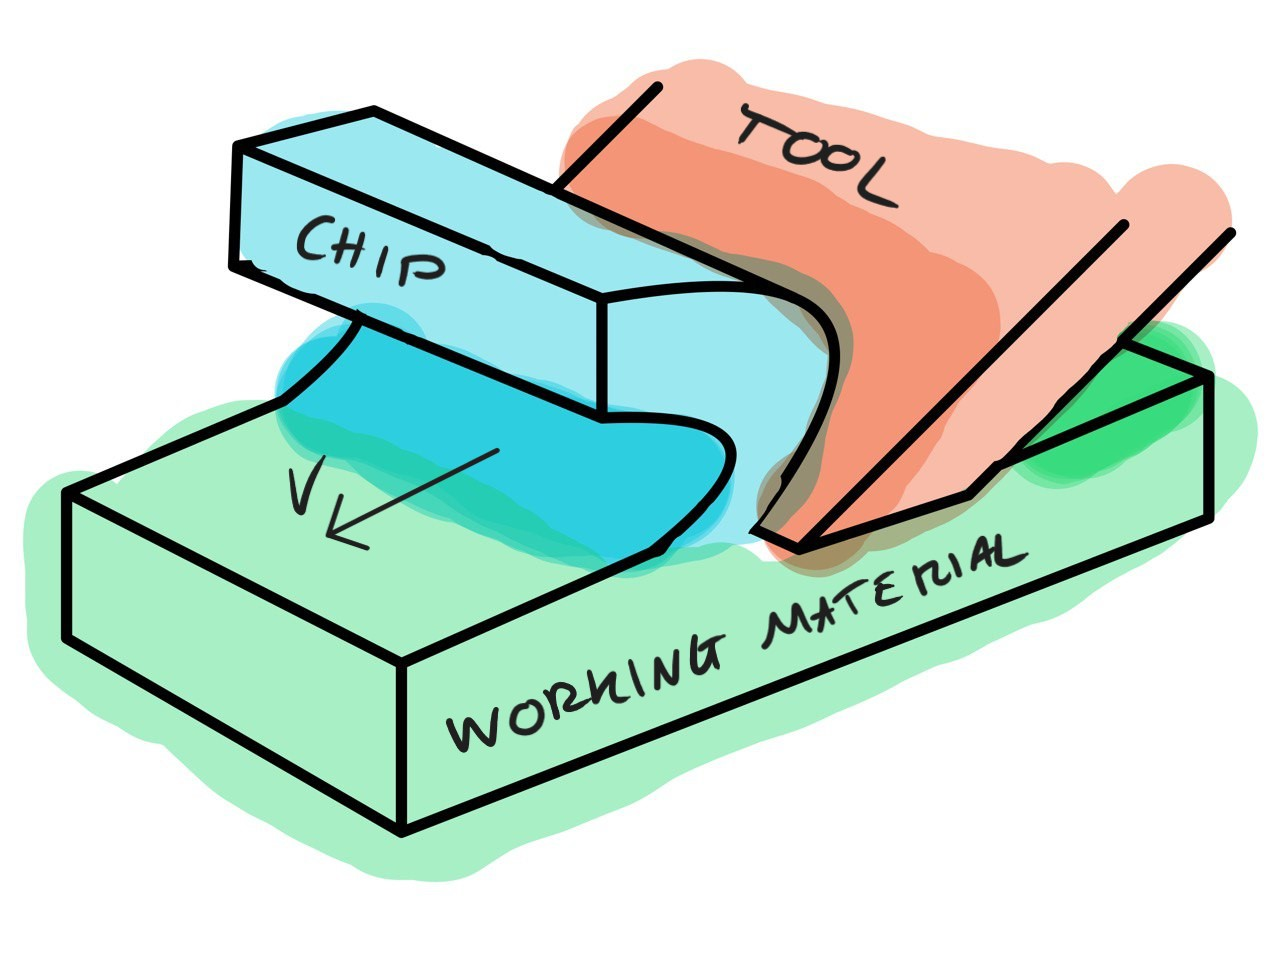
\includegraphics[width = 0.8\textwidth]{TaglioOrto}}\\
\subfloat[][\emph{Parametri del taglio ortogonale}\label{fig:TaglioOrtoParam}]
{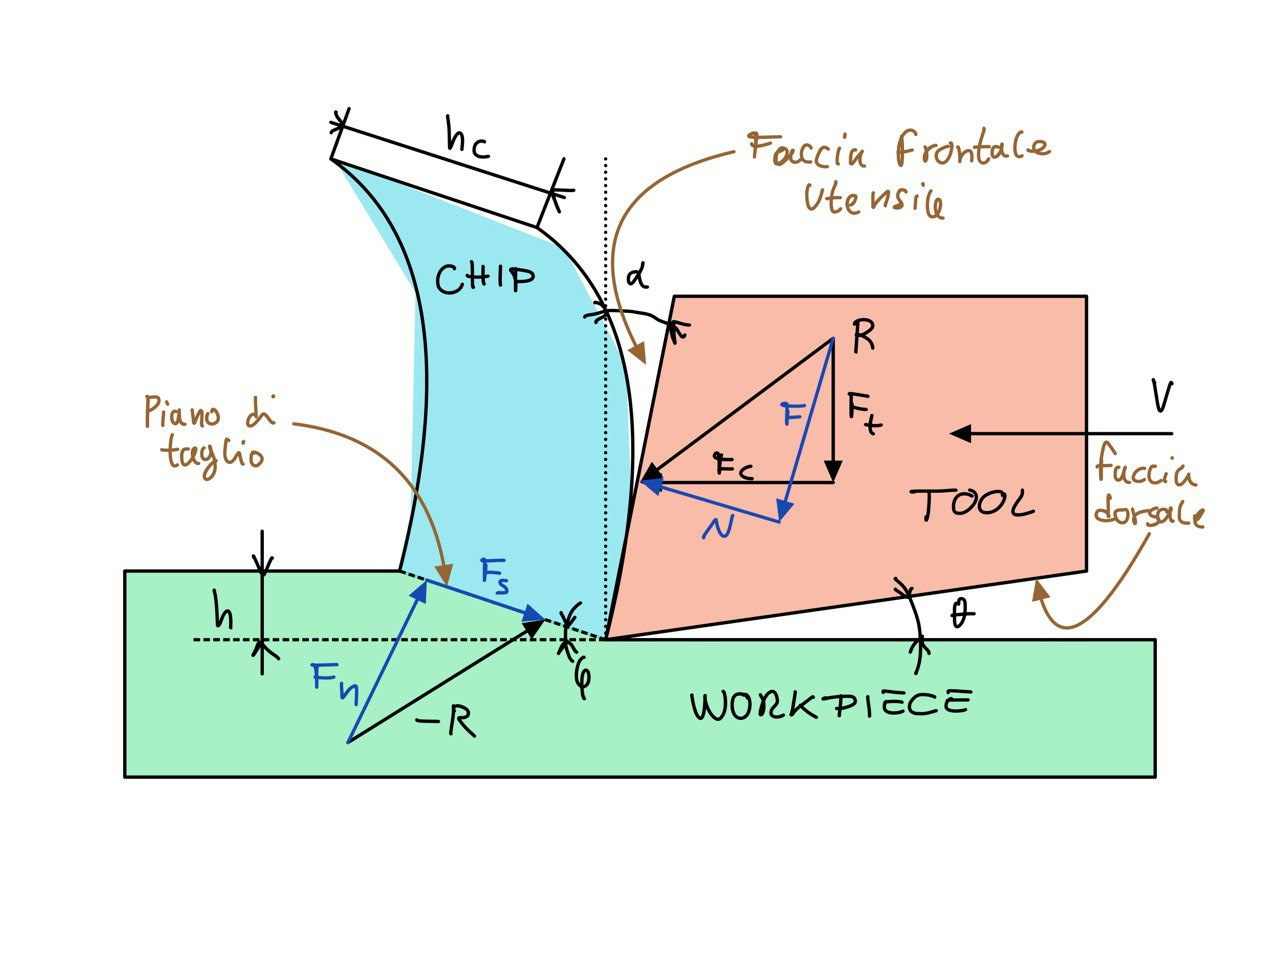
\includegraphics[width=0.7\textwidth]{TaglioOrtoScheme}}
\caption{Taglio Ortogonale}\label{fig:TaglioOrto}
\end{figure}
Si dice che il taglio è ortogonale quando la lama dell'utensile è ortogonale alla direzione della velocità di taglio.
Allora si possono definire diversi parametri come riportato nella definizione \ref{def:ParamTaglioOrto}.

\begin{definition}{Parametri del taglio ortogonale}{pramTaglioOrto}
\begin{description}
\item[$\alpha$] Angolo di spoglia superiore o frontale. Da cui
	\begin{description}
	\item[Se $\alpha > 0$] allora si dice che l'utensile ha angolo acuto,
	\item[Se $\alpha < 0$] allora si dice che l'utensile ha angolo ottuso.
	\end{description}
\item[$\theta$] Angolo di spoglia inferiore
\item[$\phi$] Angolo di taglio
\item[$h$] Spessore di taglio indeformato
\item[$h_c$] Spessore del truciolo
\end{description}
\label{def:ParamTaglioOrto}
\end{definition}

Come ipotesi ideale, si considererà che tutta la deformazione del materiale avverrà
solamente sul piano di taglio.
Allora, dai parametri del taglio ortogonale si possono ottenere:
\begin{equation}
r_c = \frac{h}{h_c} = \frac{l_c}{l} := \text{Rapporto di taglio}
\end{equation}
Dove:\\
\begin{tabular}{cl}
$l_c$ & è la lunghezza del truciolo\\
$l$ & è la lunghezza del taglio\\
\end{tabular}
\\
Mentre:
\begin{equation}
F = K \cdot A
\end{equation}
ovvero, la forza necessaria a tagliare il pezzo sarà proporzionale all'area $A$ del piano di taglio 
dovuta dalla lunghezza del piano stesso per la profondità del pezzo in senso ortogonale alla 
figura \ref{fig:TaglioOrtoParam}; in più sarà proporzionale alla pressione $K$ esercitata dall'utensile sul pezzo
Inoltre, si può intuire che: per abbassare l'intensità della forza complessiva per il taglio
sarebbe opportuno aumentare $\phi$, così da limitare l'estensione del piano di taglio e di 
conseguenza la sua area.
Si può ottenere una stima dell'angolo di taglio tramite
\begin{equation}
\tan\phi = \frac{r_c \cos\alpha}{1-r_c\sin\alpha}
\end{equation}
considerando che il rapporto di taglio lo si può misurare abbastanza facilmente dato che:
lo spessore di taglio lo si decide in base alla lavorazione da effettuare, mentre lo
spessore del truciolo lo si può misurare abbastanza facilmente.
Dunque è evidente che l'angolo $\alpha$ lo si vuole molto grande, in modo da generare piani
di taglio molto piccoli: garantendo la necessità di applicare una forza minore.

Risulta utile prestare attenzione alla successiva considerazione.
Il valore di deformazione che si raggiunge con le lavorazioni per asportazione di truciolo
è nettamente più alte che non le deformazioni per lavorazioni tramite deformazione.
Giusto per dare un'idea dell'ordine di grandezza:
\begin{equation}
\dot{\gamma} = \frac{v_s}{d} = \frac{\cos\alpha}{\cos\left(\phi - \alpha\right)} \frac{v}{d} \left[\unit{\s^{-1}}\right]
\end{equation}
nella tecnica, si osservano i seguenti valori:
\begin{description}
\item[Lavorazione per deformazione] $\approx 1 \div 10 \left[\unit{\s^{-1}}\right]$
\item[Lavorazione per asportazione] $\approx 1000 \left[\unit{\s^{-1}}\right]$
\end{description}

\subsection{Fattore di attrito}
Sappiamo che il fattore di attrito ricopre importante ruolo per quanto riguarda questo tipo
di lavorazioni. Ci si deve prestare attenzione.

\begin{equation}
\mu = \frac{\tau_i}{p}
\label{eqn:FattoreAttritoIndef}
\end{equation}
Di base, questa sarebbe la definizione principale di fattore di attrito.
Si nota che passata la tensione tangenziale di Von Misess, 
l'attrito tende a calare, nonostante nell'equazione non sia previsto tale 
comportamento.
Ciò è dovuto al fatto che per calcolare il fattore di attrito si considera un materiale
indeformabile, quando nella realtà del taglio ortogonale, non può essere.
Dunque il materiale sarà \textbf{indeformabile} fino alla tensione di Von Misess, 
passata quella bisogna considerarlo \textbf{deformabile}.
Perciò l'equazione \eqref{eqn:FattoreAttritoIndef} non descrive completamente il comportamento.
Si è sviluppato un \texttt{fattore di attrito} adatto a tale fenomeno:
\begin{equation}
m = \frac{\tau_i}{K}
\label{eqn:FattoreAttritoDef}
\end{equation}
Dove $K$ è la tensione tangenziale all'interfaccia truciolo-utensile.
Nella pratica viene preferito il fattore descritto dalla \eqref{eqn:FattoreAttritoDef} 
perché più facile da calcolare. Oltre al fatto che permette di descrivere correttamente
il fenomeno dello \eng{sticking}.

\begin{definition}{Sticking}{*}
Fenomeno di aderenza tra il truciolo e l'utensile. 
\end{definition}

\subsection{Valutazione delle forze}
Per la valutazione delle forze messe in gioco per tale lavorazione si considereranno
i tre attori separatamente e man mano sovrapponendone gli effetti.

\begin{figure}
\centering
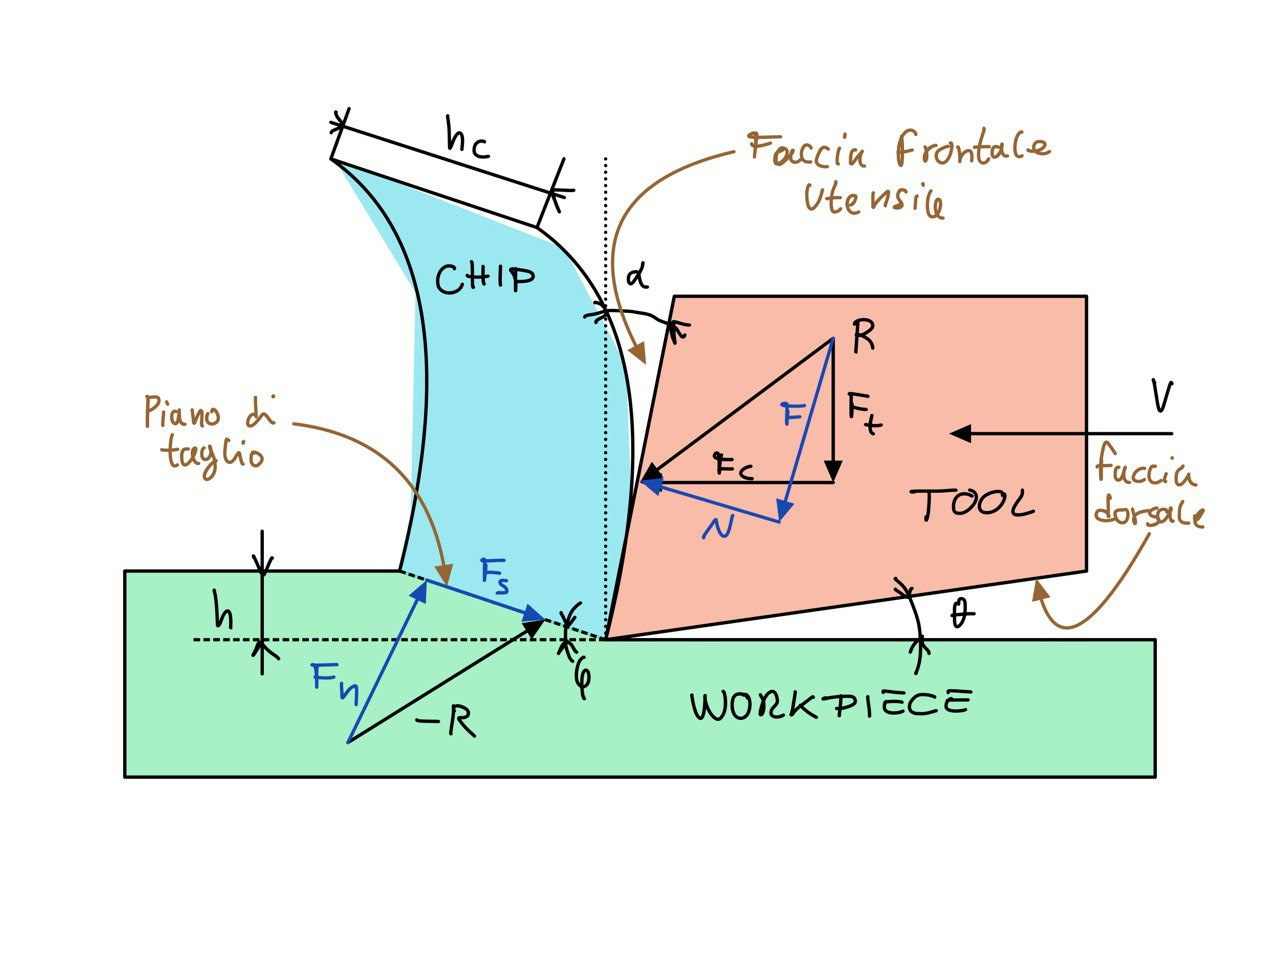
\includegraphics[width = \textwidth]{TaglioOrtoScheme}
\caption{Scomposizione delle forze per il taglio ortogonale}
\label{fig:TaglioOrtoForces}
\end{figure}

\subsubsection*{Porta utensile}
Considerando la scomposizione delle forze della figura \ref{fig:TaglioOrtoForces}.
Al porta utensile si può, operativamente, applicare una cella di carico per 
valutare la risultate applicata. Celle di carico più moderne possono eventualmente
valutare già le componenti di tale risultante.
allora possiamo ottenere i moduli delle forze:
\begin{equation}
\begin{cases}
F_c = R \cos(\alpha + \psi) &\text{Forza di taglio}\\
F_t = R \sin(\alpha + \psi) &\text{Forza di spinta dell'utensile}
\end{cases}
\end{equation}
Si possono definire ulteriori scomposizioni di forze: se prima la scomposizione
avveniva su proiezioni degli assi di riferimento rispetto al pezzo lavorato; ora si 
possono definire delle scomposizioni rispetto all'utensile.

\subsubsection*{Utensile}
Sempre in riferimento alla figura \ref{fig:TaglioOrtoForces}.
\begin{equation}
\begin{cases}
N = F_c \cos\alpha - F_t\sin\alpha\\
F = F_c \sin\alpha - F_t\cos\alpha
\end{cases}
\end{equation}
L'angolo relativo tra $R$ e $N$ viene indicato con $\beta$ e viene definito come 
\textbf{angolo d'attrito sulla faccia dell'utensile}. Vale:
\begin{equation}
\beta = \frac{F}{N} \approx \mu
\label{eqn:AngAttrito}
\end{equation}
Notare che $\beta$ è una sottospecie di coefficiente di attrito, infatti dipende
proprio da quest'ultimo.

\subsubsection*{Pezzo lavorato}
Lato pezzo lavorato si può vedere la totalità delle forze in gioco.
in particolare si devono evidenziare le forze:
\begin{description}
\item[$F_n$] risulta essere un contributo idrostatico per il materiale, dunque ne aumenta la 
duttilità. Aspetto che rende il taglio più difficoltoso. 
Ciò si risolve aumentando l'angolo del piano di taglio $\phi$ che si vedrà successivamente.
\item[$F_s$] è la vera e propria forza resistente al taglio. Si sviluppa come relazione della 
pressione di taglio resistente del materiale e l'area del piano di taglio.
\begin{equation}
F_s = k \cdot A
\end{equation}
Per rendere il taglio più agevole, si può ridurre l'area del piano di taglio nei modi che vedremo in seguito.
\end{description}

Riprendendo l'angolo del piano di taglio $\phi$, si hanno migliori condizioni lavorative
nel caso questo risulti essere molto grande.
Dalla letteratura si evidenziano le seguenti relazioni tra i vari angoli scomponenti le 
forze viste fino a prima:
\begin{subequations}
\label{eqn:Phi}
\begin{align}
\phi &= 45\unit{\degree} - \frac{1}{2}(\beta - \alpha) \label{eqn:Phi1}\\
\phi &= 45\unit{\degree} - (\beta - \alpha)\label{eqn:Phi2}
\end{align}
\end{subequations}
Sebbene indichino la relazione degli stessi parametri con due relazioni differenti \eqref{eqn:Phi}, entrambe hanno uno scopo preciso e nascono da considerazioni differenti.

\begin{description}
\item[\eqref{eqn:Phi1}] Si sviluppa partendo dalla considerazione che il sistema tenda
a consumare la minima energia.
\item[\eqref{eqn:Phi2}] Viene detta di \eng{Upper Bond}: ovvero ha l'obbiettivo di valutare
la massima forza necessaria per eseguire il taglio.
\end{description}

Per entrambi i casi risulta evidente che per aumentare $\phi$ si possono percorrere due strade:
\begin{description}
\item[$\searrow \beta$] siccome $\beta$ dipende dall'attrito tra truciolo e utensile, 
indipendentemente dallo \eng{sticking}, si può abbassare come angolo lubrificando 
l'interfaccia tra i  due.
\item[$\nearrow \alpha$] Aumentare l'angolo della faccia dell'utensile non è sempre una strada
percorribile, infatti si avrebbero utensili molto fini e fragili che tenderebbero a consumarsi
molto facilmente.
\end{description}

\begin{figure}
\centering
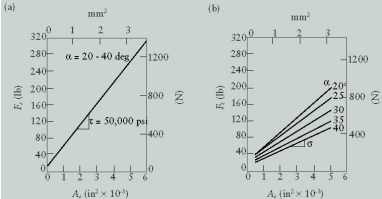
\includegraphics[width=\textwidth]{GraficiTaglioOrto}
\caption{Andamenti delle forze per il taglio ortogonale}
\label{fig:GarficiTaglioOrto}
\end{figure}

Nel grafico \ref{fig:GarficiTaglioOrto}.(a) è rappresentato l'andamento della forza di taglio 
$F_s$ giacente sul piano di taglio. Si osserva che tale forza aumenta all'aumentare dell'area 
del piano di taglio. 
Dunque è importante diminuire proprio quest'ultima: attraverso le strategie per 
aumentare $\phi$ viste in precedenza. Oltretutto tale andamento non è influenzato 
dall'angolo di spoglia superiore.
L'ipotesi che porta a tale costruzione sta nel fatto che il materiale è supposto non
incrudente. Infatti: raggiunto tale valore di sforzo tangenziale $\tau$ il materiale si 
rompe. Nel caso di materiale incrudente: si avrà una curva più che lineare, in quanto la 
deformazione porterà all'irrigidimento nella zona di taglio che necessiterà di maggiore
forza per avere la separazione del materiale.

Nel grafico \ref{fig:GarficiTaglioOrto}.(b) viene rappresentata la forza normale al piano di 
taglio $F_n$.
Questa dipende dall'angolo di spoglia superiore.
L'effetto di tale forza è stato già evidenziato: questa fornisce una specie di compressione 
idrostatica sul piano di taglio portando il materiale ad essere più duttile.
Ciò spesso si traduce in un truciolo continuo che però è problematico per la continuazione
della lavorazione: in quanto ingombrante e pericoloso.

\begin{figure}
\centering
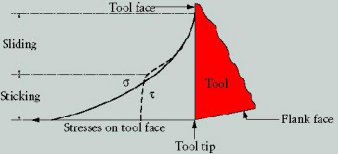
\includegraphics[width=\textwidth]{Sticking}
\caption{Tipologia di forze prementi sulla faccia dell'utensile}
\label{fig:sticking}
\end{figure}

Nel grafico \ref{fig:sticking} viene riportato il dettaglio sulla faccia superiore 
dell'utensile.
Si possono vedere due sezioni distinte:
\begin{description}
\item[\eng{Sliding}] in questa sezione si presenta lo scivolamento del truciolo sulla faccia
dell'utensile. Questo porta una cera forza resistente contro l'utensile di tipo $\tau$: ovvero 
di sforzo tangenziale. Si ha uno strisciamento completamente regolato dal coefficiente di 
attrito. Tale resistenza si annullerà nel momento in cui c'è distaccamento tra truciolo e 
faccia.
\item[\eng{Sticking}] nella zona di adesione si manifesta un particolare fenomeno per cui
il materiale del lavorato si accumula sulla punta dell'utensile. Ciò permette di generare una 
zona di ristagno che favorisce la separazione del materiale tra quello tagliato e il
truciolo. Di fatto in alcune occasioni può essere benefico per il tagliente in quanto
diventa uno strato protettivo. La resistenza portata da tale fenomeno diventa di pura 
deformazione $\sigma$. 
\end{description}

Al momento non si è ancora approfondita la finalità dell'angolo di spoglia inferiore $\theta$.
Idealmente servirebbe ad evitare lo strisciamento tra utensile e lavorato.
Siccome nella realtà bisogna considerare anche il ritorno elastico, non è possibile ottenere
un perfetto distaccamento tra utensile e lavorando. Dunque un po' di strisciamento si 
verifica in qualsiasi occasione. Ciò provoca usura dell'utensile.
Tra l'altro questo tipo di usura è la più severa per l'utensile.


\section{Taglio ortogonale realistico}
Il taglio del materiale non avviene più nel piano
di taglio, bensì sulla zona di taglio detta anche
\textbf{Zona di taglio primaria} mostrato in 
figura \ref{fig:TaglioOrtoRealScheme}.

\begin{figure}
\centering
\subfloat[][\emph{Schematizzazione del taglio ortogonale realistico}\label{fig:TaglioOrtoRealScheme}]
{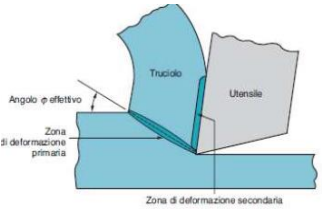
\includegraphics[width=0.5\textwidth]{TaglioOrtoRealScheme}}\\
\subfloat[][\emph{Tipologie di truciolo}\label{fig:Trucioli}]
{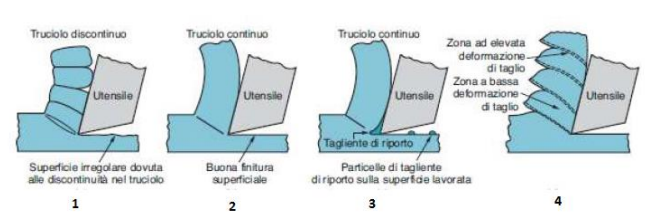
\includegraphics[width = \textwidth]{TaglioOrtoReal}}
\caption{Taglio ortogonale reale}
\label{fig:TaglioOrtoreal}
\end{figure}

Inoltre si osserva una zona deformata plasticamente, per cui si presenta un incremento della 
resistenza pari a quasi 3 volte la durezza nominale del pezzo lavorato.

Analizzando il comportamento del truciolo si possono
verificare delle situazioni, come illustrato in figura \ref{fig:Trucioli}:
\subsection{Truciolo continuo} Si verifica per velocità abbastanza basse. Come dice il nome Truciolo forma un continuo filamento di materiale.
Risulta più semplice lubrificare la faccia dell'utensile, abbassando $\beta$ come avevamo visto
in precedenza per diminuire la dimensione del piano di taglio. Dunque la zona di taglio resta più sottile
e la superficie uscirà dalla lavorazione con una 
finitura migliore.

Se da questa situazione si aumenta la velocità di
lavorazione, si va a formare una zona detta: 
\textbf{tagliente di riporto}.
Ciò è dovuto all'aumento della velocità con conseguente formazione della zona di ristagno
davanti alla faccia dell'utensile.
In particolare il tagliente di riporto:
\begin{itemize}
\item $\alpha$ aumenta per via per effetto della
zona di ristagno, per ciò si abbassa la forza di 
taglio.
\item In qualche misura protegge la faccia dell'utensile.
\item Può depositarsi sulla faccia del lavorato 
intaccandone la finitura superficiale.
\end{itemize}

Aumentando ulteriormente la velocità; la zona di taglio primario si assottiglia ulteriormente.
Comincia ad instaurarsi il fenomeno dello \eng{stiching}.
Il fenomeno si deve principalmente al riscaldamento
del materiale il quale crea adesione sulla faccia del
tagliente. Sarà, dunque, necessario aumentare la 
forza di taglio.

Si può già intuire che la velocità di taglio sarà 
strettamente legata alla temperatura generata durante la lavorazione.

Rimanendo nel tema del truciolo continuo si può verificare una situazione di truciolo continuo ma
ondulato

\subsubsection{Truciolo continuo ondulato}
È dovuto ad una variazione periodica nella forza di taglio. Possono esserci diversi motivi per cui 
si verifichi tale variazione: 
\begin{itemize}
\item Superficie rugosa, limita lo scorrimento del
tagliente.
\item Presenza di vibrazioni autoeccitate: se le vibrazioni sono dovute a forti variazioni nella superficie di taglio.
\item Distacchi del tagliente di riporto che va ad aderire alla superficie del materiale lavorato. 
Impone una maggiore forza perché l'utensile "deve"
far aderire tale riporto sulla superficie.
\item Vibrazioni forzate: generate dalla macchina 
e in genere dovute agli elementi elastici della macchina.
\item Quando si rompe il tagliente di riporto, portandosi via anche un pezzo del tagliente vero
e proprio.
\end{itemize}

Altra situazione particolare, di cui tenere nota, è la casistica in cui si forma il truciolo a dente di sega.

\subsubsection{Truciolo continuo a dente di sega}
Costituito da sezioni a diversa deformazione, la successione di zone spesse a bassa deformazione a zone fine di alta deformazione.
Le cause di tale comportamento è da imputarsi a:
\begin{itemize}
\item bassa conduttività termica del materiale,
per cui non riesce a smaltire il calore generato dalla lavorazione. 
\item Ciò spiega l'alternanza delle zone ad alta deformazione e bassa deformazione: le sezioni a bassa deformazione sono caratterizzate da un'alta temperatura relativa per cui l'utensile taglia
più facilmente il materiale. Una volta asportata una sezione di materiale, viene automaticamente smaltito
del calore "bloccato" nel materiale. Dunque la sezione successiva trova un calore minore, per cui il 
tagliente fa più fatica a tagliare e deforma di più 
il materiale. Per questo motivo le sezioni ad alta 
deformazione sono più fine.
\end{itemize}
Ultima casistica di truciolo, è quella del truciolo 
discontinuo.

\subsection{Truciolo discontinuo}
Si verifica in situazioni di velocità estremamente
basse su macchine scadenti a bassa rigidezza.
Altre situazioni per cui si va ad avere truciolo 
discontinuo sono:
\begin{itemize}
\item Per materiali che contengono inclusioni e fasi
secondarie che alzano le tensioni. Ciò provocano delle continue rotture di truciolo.
\item Situazioni di stick-slip.
\end{itemize}

Sebbene il truciolo continuo sia ricercato per favorire una finitura superficiale migliore, spesso
non è possibile tenere trucioli particolarmente lunghi. Durante la lavorazione un truciolo lungo
può essere d'intralcio all'operatore e alla macchina.

Allora si ha la necessità di rompere il truciolo.

\begin{wrapfloat}{figure}{O}{0pt}
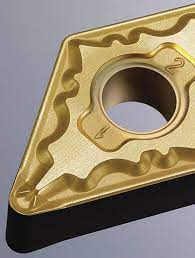
\includegraphics[width = 0.3\textwidth]{Rompitruciolo}
\caption{Esempi di rompi-truciolo}
\label{fig:Rompitruciolo}
\end{wrapfloat}


\subsection{La rottura del truciolo}
È particolarmente facile coi materiali fragili, più
complicato per quei materiali duttili che tendono
a formare dei trucioli continui.
Allora si ricorre a opportuni \textbf{rompi-truciolo},
inserti che possono essere fissati all'utensile o già
disegnati su esso, per favorire la rottura del 
truciolo ponendo ulteriore deformazione al materiale
asportato.
I rompi-truciolo hanno uno specifico valore efficace
di rottura del truciolo dipendente dalla profondità 
dello spessore indeformato: questa è una 
caratteristica della forma e dimensione geometrica 
del rompi-truciolo. In figura \ref{fig:Rompitruciolo} 
un dettaglio.

\section{Taglio obliquo}
Viene sfruttato maggiormente dalle aziende.
Garantisce una lavorazione che necessita di maggiore
forza per il taglio, ma la vita del utensile
è più lunga.

A differenza del taglio ortogonale dove si veniva
a formare un truciolo continuo a forma di spirale.
Nel taglio obliquo si forma un truciolo a forma 
elicoidale, che ha una propria tendenza geometrica
a spostarsi via dal punto di lavorazione.
Si evita la necessità di rompere il truciolo, anche 
se è una pratica che comunque viene mantenuta.
È opportuno definire un nuovo angolo di spoglia 
superiore.
\begin{align}
\alpha_e &:= \text{Angolo di spoglia efficace}\\
\alpha_n &:= \text{Angolo di spoglia normale}\\
&\text{In generale: }\alpha_e > \alpha_n
\end{align}
Vale che più il tagliente è inclinato, più aumenta $\alpha_e$ 
e di conseguenza $F_c$ diminuisce.

Nel caso in cui il tagliente non sia più grande del
pezzo in lavorazione, lo spessore del truciolo 
indeformato non è più sufficiente a descrivere i 
fenomeni legati a questo. Dunque è necessario parlare
di \textbf{avanzamento} $f$. Inoltre si introduce 
la \textbf{profondità di passaggio} $w$.

\begin{figure}
\centering
\subfloat[][\emph{Schema del taglio obliquo}\label{fig:TaglioObliquoScheme}]
{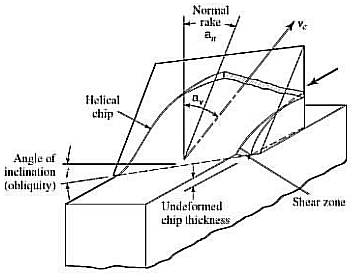
\includegraphics[width = \textwidth]{TaglioObliquo}}\\
\subfloat[]
[\emph{Parametri del taglio ortogonale per confronto}\label{fig:TaglioObliquoParam1}]
{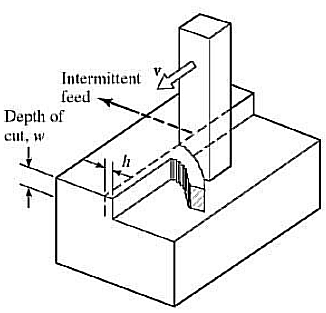
\includegraphics[width = 0.4\textwidth]{TaglioObliquoParam1}}\quad
\subfloat[][\emph{Ulteriori parametri del taglio obliquo}\label{fig:TaglioObliquoParam2}]
{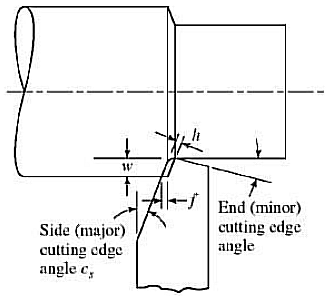
\includegraphics[width = 0.4\textwidth]{TaglioObliquoParam2}}
\caption{Il taglio obliquo}
\label{fig:TaglioObliquo}
\end{figure}

\subsection{Tornitura}
Un esempio di tornitura è riportato alla figura \ref{fig:TaglioObliquoParam2}.
\begin{wrapfloat}{figure}{O}{0pt}
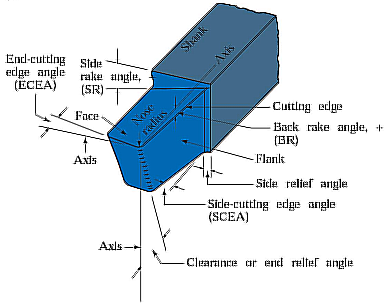
\includegraphics[width = 0.5\textwidth]{Utensile}
\caption{Esempio di utensile per tornitura}
\label{fig:UtensileTornitua}
\end{wrapfloat}

\begin{itemize}
\item utensile con tagliente inclinato
\item $f$ è ortogonale al tagliente e rappresenta 
l'avanzamento;
\item $w$ è la profondità di passata
\item $h$ è lo spessore di truciolo indeformato.
\end{itemize}

Con l'utensile inclinato si ha una maggiore forza 
necessaria al taglio, però si aumenta 
considerevolmente la durata dell'utensile.
Indubbiamente la caratterizzazione del tagliente 
risulta più complicata. Si ha l'ulteriore vantaggio
di avere un utensile che può presentare più 
taglienti.

\subsection{Calcolo della forza ed energia}
Siccome per via del tipo di lavorazione non siamo in grado di sfruttare
la deformazione per flusso plastico a causa della velocità decisamente 
superiore.
È decisamente importante sapere quanta energia o potenza è necessaria 
per effettuare la lavorazione. Perché tale potenza sarà quella che il
motore della macchina deve fornire all'utensile.

A differenza della lavorazione per deformazione plastica in cui 
la "pressa" deve fornire una certa pressione per permettere la 
deformazione. Nell'asportazione si possono cambiare alcuni
parametri in base anche punto della lavorazione si è.
Continuando a lavorare il pezzo.

Resta evidente come la parametrizzazione della lavorazione sia
definitivamente importante: in modo da garantire la continuazione
della lavorazione, cambiando alcune condizioni senza interromperla.
Anche per il fatto che fermando la lavorazione peggiora la finitura.

Nella definizione dell'energia necessaria si sa che si va a commettere
un'errore di circa il $20\%$.
Di fatto sarebbe necessario conoscere $\beta$, ma non è facile da valutare.
Allora si può valutare la \textbf{pressione di taglio}.

\begin{equation}
p_c = \frac{\overbrace{F_c}^{\text{Componente parallela alla velocità di taglio}}}{h \cdot w}
\end{equation} 
Per ottenere una forma di energia basta integrare la pressione
o forza per la lunghezza del lavoro eseguito ovvero:
\begin{equation}
l := \text{lunghezza di taglio}\\
\end{equation}

\begin{definition}{Pressione ed energia di taglio specifica}{PEspec}
\begin{subequations}
\begin{align}
p_c &= \frac{F_c}{h \cdot w} \\
E_1 &= p_c \cdot \frac{l}{l} \:[\unit{\W\s/\m^3}]
\end{align}
\end{subequations}
Dove $p_c$ è la pressione specifica di taglio e $E_1$ è l'energia specifica.
\end{definition}

\begin{definition}{Fattore di rimozione}{FattRim}
Si può definire anche il Fattore di rimozione del materiale:
\begin{equation}
k_1 = \frac{1}{E_1}
\end{equation}
dove $k_1$ rappresenta la quantità di materiale asportato da una macchina
a motore a potenza unitaria.
\end{definition}

I 3 parametri non sono costanti per un materiale perché dipendono anche dai
parametri di processo quali spessore di truciolo indeformato, angolo di spoglia e
velocità di taglio.
L'energia spesa nella zona di taglio primaria e la quantità di materiale rimosso
sono proporzionali allo spessore di truciolo indeformato.
\begin{equation}
E = k \cdot h \cdot p \cdot l
\end{equation}

Nella zona di taglio primaria la pressione specifica, l'energia specifica e il fattore di
rimozione del materiale sono costanti del materiale.
L'energia consumata sul dorso dell'utensile è indipendente dallo spessore di
truciolo indeformato, possiamo ritenerla quasi costante.
Quindi vale:
\begin{equation}
\frac{E_d}{h \cdot p \cdot l} \neq cost.
\end{equation}

A questo punto si è definita una relazione in cui si può già definire la forza necessaria.
C'è da tenere in considerazione l'usura dell'utensile: in quanto quest'ultima tende
a richiedere una maggiore pressione da parte del tagliente per tagliare.
Siccome l'usura del tagliente è un argomento che richiede la considerazione di diversi
parametri e che tali non possono sempre essere determinatiti così facilmente.
Semplicemente si aggiunge un $30\%$ in più all'energia necessaria.

Ulteriori parametri derivati dai precedenti sono:
\begin{definition}{Ulteriori Parametri}{UltParam}
Sono delle derivazioni dei parametri visti precedentemente.
\begin{equation}
E = E_1 \left(\frac{h}{h_{ref}}\right)^{-a} = E_1 \cdot h^{-a}
\end{equation}
Dove $E$ è l'energia di lavorazione, $h_{ref} = 1\unit{\mm}$ è lo spessore indeformato di 
riferimento e $a \approx 0.3$.
Da cui si può definire la potenza necessaria per la lavorazione:
\begin{equation}
Power(W) = \frac{E \cdot V_t}{\eta}
\end{equation}
Dove $V_t$ è la velocità di taglio, $\eta$ il rendimento della macchina.
Da cui si può ottenere la forza necessaria per il taglio:
\begin{equation}
F_c = \frac{Power(W)}{v}
\end{equation}
\end{definition}

\subsection{Temperature}
Siccome la lavorazione prevede di "muovere" del materiale dentro se stesso
questo provoca un accumulo di energia danti alla faccia dell'utensile.
Tale energia rimane nella maggior parte nel truciolo.

\begin{wrapfloat}{figure}{I}{0pt}
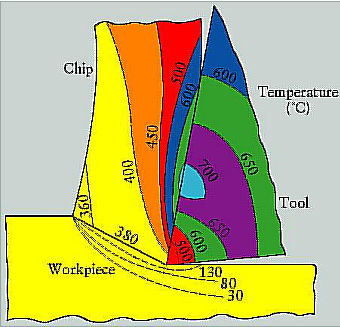
\includegraphics[width = 0.4\textwidth]{Temperature}
\caption{Analisi termica dell'asportazione di truciolo}
\label{fig:Temp}
\end{wrapfloat}

Come si vede dalla figura \ref{fig:Temp}, le temperature raggiunte non sono da 
trascurare: si può arrivare a $\approx 1000\unit{\celsius}$ sulla faccia dell'utensile.
Sappiamo che con l'aumento della temperatura, aumentano il numero di dislocazioni
interne al materiale che diventa più duttile dunque più facile da lavorare.

La maggior parte dell'energia resta interna al truciolo che, portando con se del
calore, abbassa la temperatura del lavorato. Resta il calore trasferito 
all'utensile, il quale tende ad aumentare la temperatura considerevolmente.
Infatti, come si vede proprio dalla figura \ref{fig:Temp}, è proprio
l'utensile a mostrare le temperature più alte. Ciò impone che il
materiale dell'utensile debba essere di un materiale alto resistente a caldo.

\begin{figure}
\centering
\subfloat[][\emph{Schema delle isoterme sulla faccia dell'utensile}\label{fig:TempUtensile}]
{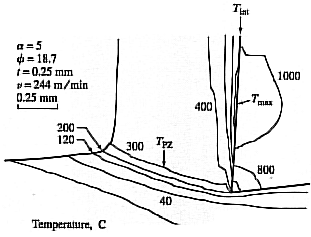
\includegraphics[width = 0.4\textwidth]{TempScheme}}\quad
\subfloat[][\emph{Relazione tra velocità di lavorazione e temperatura}
\label{fig:TempVel}]
{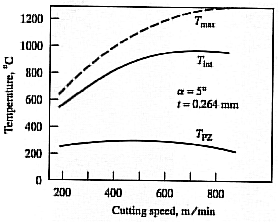
\includegraphics[width = 0.4\textwidth]{TempVel}}
\caption{Temperature durante le lavorazioni ad asportazione}
\label{fig:TempLav}
\end{figure}

Come fatto in precedenza, si è cercato di relazionare la temperatura con la
velocità di lavorazione: legame che fisicamente è noto ma non così facile 
da porre analiticamente.

\begin{equation}
T_t = E \left( \frac{v \cdot h}{k \cdot \rho \cdot c}\right)^{1/2}
\end{equation}
Dove:\\
\begin{tabularx}{\textwidth}{cX}
$E_1$ & Energia specifica\\
$v$ & Velocità di taglio\\
$h$ & Spessore di truciolo indeformato\\
$k$ & Conduttività termica\\
$\rho$ & Densità\\
$c$ & Calore specifico 
\end{tabularx}\\
Se ne ottiene una stima della temperatura media sulla faccia dell'utensile.
Come spesso succede nei sistemi fisici reali, tutta l'energia donata dalla
macchina al materiale viene trasformata in calore.
Indubbiamente durante le lavorazioni non si deve superare la temperatura di fusione
del materiale lavorato: altrimenti si va ad ottenere una lavorazione molto grossolana di
cui non si riesce a controllarne i parametri.
I materiali a bassa fusione risultano più facili da lavorare.
Inoltre, per lavorazioni di finitura particolarmente restrittive, bisogna considerare
le variazioni dimensionali dovute alla dilatazione termica.

\subsection{Fluidi da taglio}
In industria ed artigianato, queste lavorazioni vengono spesso
effettuate con l'assistenza dei fluidi da taglio.
Questi hanno diverse funzioni per la lavorazione, tipo:

\begin{description}
\item[Lubrificazione] si cerca di abbassare l'attrito nella
lavorazione, per favorire un'asportazione più agile.
Il problema sta nel portare il fluido nella zona di lavorazione,
impedito del movimento del truciolo.
Perciò aumentando la velocità di lavorazione di ha una 
lubrificazione meno efficacie.
\item[Raffreddamento] Diminuendo la temperatura sulla faccia 
dell'utensile si può lavorare a velocità più alte.
Al contempo questo rappresenta un problema: se l'utensile non è 
costantemente immerso nel materiale, il raffreddamento potrebbe
diventare uno shock termico per via delle forti variazioni di 
temperature.
\item[Rimozione del truciolo] Utilizzando dei sistemi ad alta
pressione si possono sfruttare gli utilizzi precedenti mentre 
si spostano i trucioli dalla zona i lavorazione.
\end{description}ù

I principali metodi per l'applicazione dei fluidi da taglio sono:
\begin{itemize}
\item Oliatore manuale o in pasta,
\item Sistemi ad alta pressione,
\item Attraverso gli utensili,
\item Mediante ugelli e sistemi di ricircolo e filtraggio,
\item Applicazioni a nebbia.
\end{itemize}

I fluidi da taglio hanno dei problemi in termini di smaltimento!
Per cui spesso si lavora a secco o se ne usa il meno possibile.

\subsection{L'usura degli utensili}
\textbf{Premessa}: quando si parla di processi a deformazione si considera maggiormente come causa dell'usura pressione e forza.
In genere l'usura arriva a 100000 pezzi prodotti, rendendolo un aspetto secondario nella scelta della lavorazione.
Per l'asportazione di truciolo si hanno utensili che presentano una vita molto più breve. Si va dai 10 minuti, a qualche ora.
Ovviamente ciò implica molti fermi macchina che si rendono evidenti sulla finitura superficiale.
L'usura dipende dal materiale dell'utensile che può avere diverse specifiche forme.

\begin{definition}{Usura}
perdita di materiale da parte dell'utensile. Può essere
\begin{description}
\item[Progressiva] dovuta allo strisciamento tra materiale e utensile.
\item[Istantanea] dovuta a distacchi improvvisi di materiale per diversi motivi quali: distacco del tagliente di riporto, vibrazioni ecc\dots
\end{description}
\end{definition}

\begin{description}
\item[Usura del dorso] si manifesta sul dorso dell'utensile dovuto allo strisciamento tra utensile e lavorato.
\end{description}
L'effetto è quello di perdere il controllo sulle tolleranze ottenute nella lavorazione, peggiorando di fatto la finitura.
Consumando il tagliente, automaticamente, aumentano le forze necessarie per separare il materiale.

I parametri di riferimento sono:\\
\begin{tabular}{cl}
$V_B$ & valore medio dell'estensione delle striature sul dorso dell'utensile\\
$V_{B_{max}}$ & massima estensione delle striature dovute all'utensile.\\
\end{tabular}\\
Vengono identificati come in figura \ref{fig:StriaturaUsura}.
La variazione di questi parametri dipende fortemente dalla velocità: più alta è la velocità di taglio, più bassa è la durata dell'utensile.
Si può vedere alla figura \ref{fig:DurataUsura}.

\begin{wrapfloat}{figure}{O}{0pt}
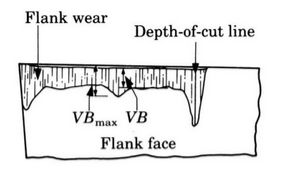
\includegraphics[width = 0.4\textwidth]{StriatureUsura}
\caption{Titpiche striature dovute all'usura}
\label{fig:StriaturaUsura}
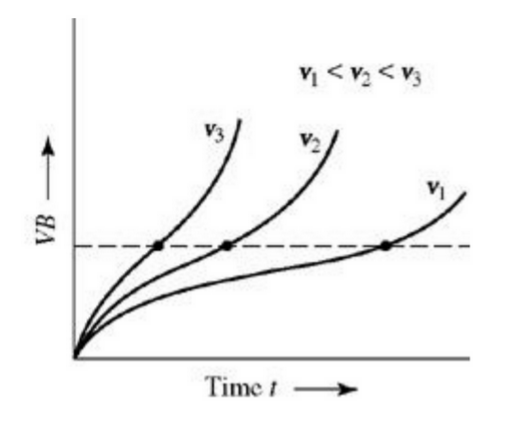
\includegraphics[width = 0.4\textwidth]{DurataUsura}
\caption{Velocità di generazione delle striatura, indice dell'usura dell'utensile. Vale che $v_1 < v_2 < v_3$}
\label{fig:DurataUsura}
\end{wrapfloat}

\eng{Depth of cut line} ovvero l'usura dentale.
La zona dell'utensile che viene a contatto con la superficie del lavorato si consuma più velocemente per la possibilità della presenza di ossidi sulla superficie.

\subsubsection{Usura della faccia}
Le alte temperature possono formare delle \textbf{craterizzazioni} sulla faccia del dorso dovuta ad abrasioni e strisciamenti dei trucioli.
Non è critica come l'usura del dorso. Si definisce:
\begin{equation}
KT := \text{caratterizzazione del cratere che si forma sulla faccia}
\end{equation}
La misurazione è riportata alla figura \ref{fig:Craterizzazione}.
Può essere un problema più per le finiture che per le sgrossature.

L'arrotondamento del naso dell'utensile è una forma di usura. Va considerato sopratutto in termini di finitura superficiale, in quanto si vedrà, essere caratterizzante per la finitura superficiale.
Le forme di usura dipendono dal materiale dell'utensile.

\begin{figure}
\centering
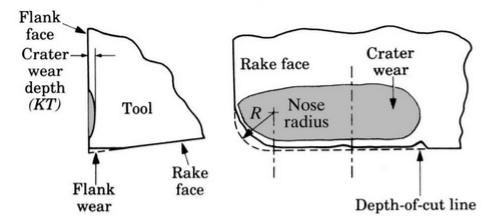
\includegraphics[width = \textwidth]{Craterizzazione}
\caption{Caratterizzazione della craterizzazione sulla faccia dell'utensile}
\label{fig:Craterizzazione}
\end{figure}

In genere è difficile misurare lo stato di usura di un utensile nell'ambito industriale.
Dunque ci si basa sulla previsione dell'usura.
Oppure si valutano operazioni di finitura, in cui al peggioramento della lavorazione si valuta l'usura.
Analogamente per la sgrossatura in finzione del materiale asportato.

\subsubsection{Previsione della durata dell'utensile}
La previsione della durata è critica: se si coordina correttamente la durata dell'utensile con la durata della lavorazione, si può evitare di interrompere la lavorazione. Ciò si vedrebbe sulla superficie del lavorato.
Come parametri da considerare per la previsione troviamo:
\begin{itemize}
\item L'usura cresce con la distanza percorsa dall'utensile
\item La durata cala con la velocità di taglio:
\begin{equation}
\text{Se } V = cost. \Rightarrow d = cost. \times t
\end{equation}
\item La velocità d'usura cresce con la temperatura.
\item La temperatura cresce con la velocità di taglio.
\end{itemize}

Allora nel tempo si è sviluppata la \textbf{Formula di Taylor}:
\begin{equation}
V \times t^n = C \label{eqn:FormulaTaylor}
\end{equation}
Dove:\\
\begin{tabular}{cl}
$n$ & dipende dal materiale dell'utensile\\
$C$ & dipende dal materiale del lavorato
\end{tabular}
All'epoca di Taylor non esistevano tutti i materiali per utensili sono in uso oggi. Dunque le relazioni non vanno sempre bene e, alle volte, sono troppo semplicistiche rispetto al metodo di usura per materiali moderni.
Anche la tecnologia abbordo macchina era completamente diversa per cui utensili usati oggi hanno, in generale, durata maggiore.

\begin{wrapfloat}{figure}{O}{0pt}
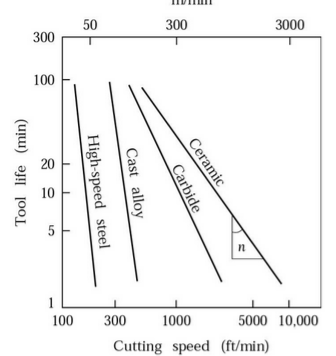
\includegraphics[width = 0.4\textwidth]{GraficoTaylor}
\caption{Grafici della formula \eqref{eqn:FormulaTaylor} per diversi materiali}
\label{fig:GraficoTaylor}
\end{wrapfloat}

Giusto per dare un'idea degli ordini di grandezza ecco alcuni esempi di parametri:
\begin{align}
\begin{cases}
\text{HSS: } &n = 0.1 \div 0.25\\
\text{Carburi} &n = 0.25 \div 0.4\\
\text{Ceramici} &n = 0.4 \div 0.7  
\end{cases}
\end{align}
Dalla formula \eqref{eqn:FormulaTaylor} si osserva che all' aumentare di $n$ la vita dell'utensile cala in maniera meno critica.

Lo \eng{stiching} modifica la velocità di usura aumentandone la durata per via della sorta di protezione della faccia di spoglia superiore.
Aumentando le temperature d'esercizio migliora la vita (grazie ai materiali che mantengono durezza elevata ad alta temperatura) per via del fatto che il materiale lavorato risulterà rammollito.

Allora si è sviluppata una formula alternativa della formula di Taylor che si adatta meglio ai tempi moderni.
\begin{equation}
t = \frac{K}{v^{1/n}} \Rightarrow t = \frac{K}{v^{1/n_1} f^{1/n_2} w^{1/n_3}} \label{eqn:TaylorModerno}
\end{equation}
In cui di solito vale che $n_1 < n_2 < n_3$ che per un acciaio rapido vale;
$n_1 = 0.1, \, n_2 = 0.18, \, n_3 = 0.45$
Per cui si può osservare che dalla formula \eqref{eqn:TaylorModerno} la durata dell'utensile cala all'aumentare della velocità con un fattore 10.
Infatti, $\frac{1}{n_1} = 10, \, \frac{1}{n_2} = 5.5, \, \frac{1}{n_3} = 2.2$
Allora conviene modificare, come parametri in base alla loro influenza, proprio $w$ e $f$ perché la durata del utensile risulta meno sensibile a questi.

Ci sono dei casi che non sono prevedibili tramite le formule di Taylor \eqref{eqn:FormulaTaylor} e \eqref{eqn:TaylorModerno}:
\begin{itemize}
\item Rottura per schianto dell'utensile se di materiale molto fragile;
\item Il comportamento statistico del materiale andrebbe considerato.
\end{itemize}

Alcune soluzioni migliorative possono essere:
\begin{itemize}
\item Addizione tra l'utensile e materiale radioattivo, che attraverso la misura delle radiazioni è possibile stimare quanto si sia consumato.
\item Misurazione della coppia resistente per valutare l'usura. Ciò è valido solamente se la lavorazione è sempre uguale.
\end{itemize}

\subsection{Qualità della superficie prodotta}
\begin{quote}
Come si può misurare la qualità della superficie?
\end{quote}

\begin{itemize}
\item Rugosità superficiale
\item Tolleranze geometriche
\item Tolleranze dimensionali
\item Trasformazioni indesiderate del materiale
\item Tensioni residue sia di compressione che di trazione 
\item Formazione di cricche
\end{itemize}

\subsubsection{Rugosità superficiale}
In condizioni ideali la rugosità del materiale dovrebbe essere 0.
Picchi e avvallamenti nel materiale sono misurabili tramite $R_t$ ovviamente si presentano.
Allora:
\begin{equation}
R_t = \frac{f^2}{8R}
\end{equation}
Con $R$ è il raggio di raccordi del naso dell'utensile.
In più:
\begin{equation}
R_a \approx \frac{f^2}{32R}
\end{equation}
Le situazioni che in generale peggiorano la rugosità superficiale sono ad esempio: la rugosità stessa del materiale di partenza, tagliente di riporto ed eventuali distaccamenti, tolleranze nella geometria dell'utensile, strappi per rottura del truciolo, cricche trasversali, vibrazioni, usura utensile.
Per la finitura, l'usura dell'utensile viene decretata da quando la finitura non raggiunge le caratteristiche richieste.

\begin{wrapfloat}{figure}{O}{0pt}
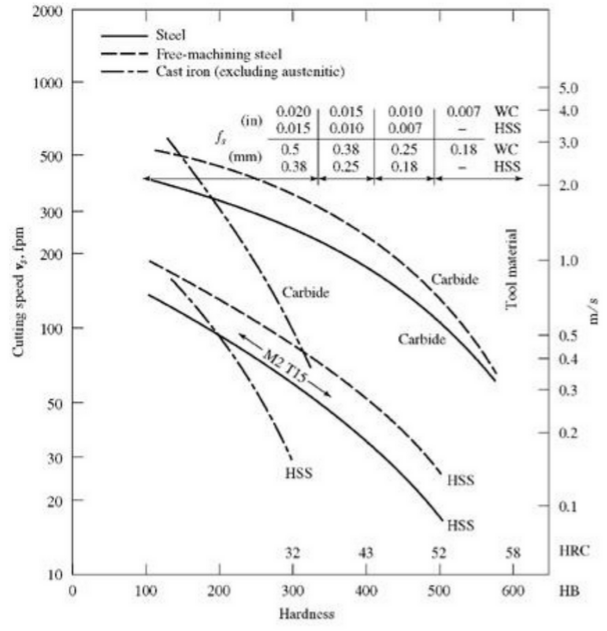
\includegraphics[width = 0.4\textwidth]{FinituraSuperficiale}
\caption{Indicazioni di velocità di taglio e avanzamento in funzione della durezza del materiale lavorato e di diversi utensili}
\label{fig:FinituraSuperficiale}
\end{wrapfloat}

\begin{example}{Esempio di valutazione dell'avanzamento}
Considerando di lavorare un acciaio automatico con utensile in carburo di tungsteno, usando il grafico \ref{fig:FinituraSuperficiale} per raggiungere un livello di rugosità $R_a = 1.6\unit{\um}$ e con una profondità di passata $w = 3.8\unit{\mm}$.
\begin{align*}
f &= \frac{0.5\unit{\mm}}{2} \: \text{In finitura si ipotizza di dimezzare l'avanzamento}\\
R_a &\approx \frac{f^2}{32R} \Rightarrow R = \frac{f^2}{32 R_a}\\
R &= 0.78\unit{\mm} \rightarrow R_{real} = 1\unit{\mm}
\end{align*}
Scegliendo un utensile con raggio di raccordo più grande si migliora la rugosità.
\end{example}

\subsection{Lavorabilità}
La lavorabilità è un concetto che convoglia diversi parametri che sono emersi nelle trattazioni precedenti.
In generale si dice che un materiale quando:
\begin{itemize}
\item Quanto facilmente si possono ottenere componenti a basso costo
\item Basse forze,
\item Basso costo di lavorazione.
\end{itemize}

In generale si definiscono delle \textbf{scale di lavorabilità} per cui vengono fatte delle prove tecnologiche per confrontare i diversi materiali.
Ad esempio:
\begin{itemize}
\item Si considera una lavorazione di riferimento: la tornitura,
\item L'utensile deve durare 60 minuti prima che raggiunga determinati valori di $WB$ o $WB_{max}$.
\item Si valuta quale materiale può essere lavorato a più alta velocità.
\end{itemize}

\begin{wrapfloat}{figure}{O}{0pt}
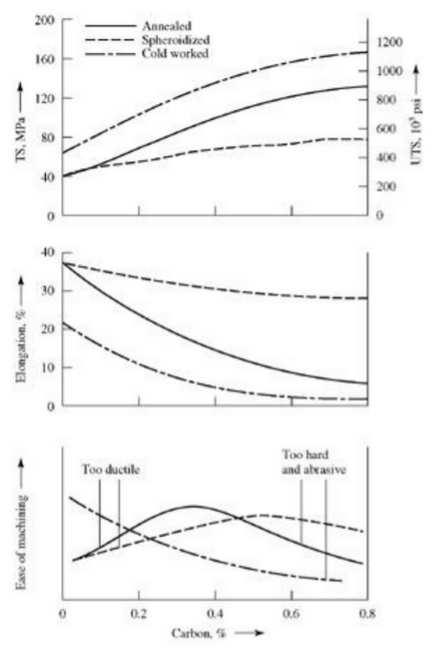
\includegraphics[width = 0.4\textwidth]{AcciaCarbonio}
\caption{Caratteristiche meccaniche utili alla lavorabilità per la lavorabilità in asportazione}
\label{fig:AcciaiCarbonio}
\end{wrapfloat}

Se si impone la velocità di taglio e si vuole valutare la lavorabilità allora si va a valutare il consumo dell'utensile.
Come si può vedere esistono diverse prove tecnologiche.

I materiali fragili o con punto di fusione basso vengono considerati dei materiali con buona lavorabilità.

In generale meglio che il materiale del lavorato non sia chimicamente reattivo, così da non reagire col materiale.

Materiali con particelle dure sono considerati meno lavorabili, per via del fatto che generano urti contro i taglienti per cui si rischia distacchi dell'utensile.
Materiali altamente termoconduttivi sono preferiti in modo da smaltire il calore accumulato sull'utensile.

Alcune soluzioni migliorative prevedono di aumentare la temperatura davanti all'utensile in modo da rendere il materiale del lavorato più cedevole.
Di certo si aumenta la probabilità di diffusione sull'utensile.

Ora si vedrà una disamina dei vari materiali maggiormente lavorati per asportazione di truciolo.

\subsubsection{Acciai al carbonio}
Hanno un'ampia gamma di durezze possibili. Si possono trovare allo stato ricotto, lavorati a freddo o induriti per precipitazione per soluzione solida.

\subsubsection{Acciai automatici}
Sono acciai contenenti due elementi che ne aumentano la lavorabilità:
\begin{description}
\item[Pb] Punto di fusione basso, evita che si formi lo sticking e proteggere l'utensile
\item[S] i solfuri di manganese, in forma globulare favorisce la rottura del truciolo.
\end{description}

\subsubsection{Acciai legati}
La resistenza meccanica aumenta rispetto ai precedenti, provocando usura accelerata dell'utensile.
Potrebbe essere possibile una ricottura per aumentare la lavorabilità.
Spesso ottenuti per sinterizzazione per cui la porosità può causare urti dell'utensile col materiale. Si può ignorare questo effetto nel caso la densità sia superiore al $90\%$ rispetto a quella vera.

\subsubsection{Acciai inossidabili}
Sono caratterizzati da scarsa lavorabilità in particolare gli austenitici e martensitici.

\subsubsection{Ghise}
Sono abbastanza lavorabili per via delle lamelle di grafite fragili delle ghise grigie. Per le altre la lavorabilità è abbastanza buona.

\subsubsection{Zinco e Magnesio}
Da prestare attenzione al punto di fusione abbastanza basso. Sono molto rigidi per cui godono di una buona lavorabilità.
Il magnesio alle alte temperature può bruciare.

\subsubsection{Alluminio}
Più lavorabile se incruditi per abbassare la lavorabilità anche in caso di invecchiamenti e \ac{TT}.

\subsubsection{Rame}
Come per l'alluminio anche il rame deve essere trattato per abbassare la duttilità altrimenti tende ad impastare l'utensile.

\subsubsection{Nichel e superleghe}
Ottime resistenze meccaniche anche ad alte temperature, per cui queste leghe sono particolarmente difficili da lavorare anche per asportazione.

\subsubsection{Titanio}
Si tratta di un materiale particolarmente fragile, per cui ben lavorabile per asportazione di truciolo.

\subsection{Materiali per utensili}
L'evoluzione dei materiali ha portato ad una migliore resa di materiali adatti per utensili. Anche le macchine hanno visto una forte evoluzione che porta a sfruttare al meglio le proprietà dei nuovi materiali.

Ricordando che:
\begin{description}
\item[Resilienza] è la capacità del materiale di assorbire istantaneamente energia meccanica prima che il materiale giunga a rottura.
\item[Tenacità] è la capacità del materiale a resistere sollecitazioni meccaniche nel tempo.
\end{description}
Dovrebbe essere che l'utensile sia più duro del materiale da lavorare.
In più si cercano dei materiali che offrano maggiore resistenza, maggiore durata e minore deformazione plastica dell'utensile.
Anche la resistenza agli shock meccanici è molto apprezzata.
Sempre di questo passo, si ricerca una certa resistenza agli shock termici nei casi in cui l'utensile non è costantemente immerso nel materiale da lavorare. Anche se il materiale può offrire alta conducibilità termica viene apprezzato, in modo da smaltire il calore accumulato sulle facce dello stesso.
Nei casi in cui ci sia adesione tra utensile-lavorato è necessario:
\begin{itemize}
\item bisogna evitare la saldatura tra i due e che eventualmente ci sia diffusione.
\item Si può favorire l'adesione per garantire una sorta di protezione delle facce.
\end{itemize}
In generale si osserva che alcuni materiali che resistono ad alta temperatura presentano comunque una bassa resilienza ad alta temperatura.

Ora si avrà una disamina dei principali materiali usati per tale scopo.

\subsubsection{Acciai Ipereutettoidici}
Si favorisce la formazione della fase martensitica nell'acciaio.
Offrono un primo rammollimento già a $250\unit{\celsius}$
Per cui vengono utilizzati per lavorare materiali particolarmente teneri a bassa velocità.
In generale possono avere $\alpha>>0$ e si possono riaffilare.
\subsubsection{Acciai HSS}
Possono essere con matrici a base di \textbf{carburi di molibdeno} o \textbf{carburi di tungsteno}.
Come temperatura limite di lavorazione si attesta attorno a $550\unit{\celsius}$.
Sono ottenuti per deformazione plastica a caldo e poi \ac{TT} e in fine la rettifica per affilarli.
Offrono una buona resilienza e possono essere riaffilati.
I \ac{TT} servono per ottenere ossidazione di $Fe_3O_4$ e nitruri (più apprezzati) o carburi di titanio.
Si fanno per ottenere una durezza da 2 o 6 volte più grande.
\subsubsection{Acciai per colata}
Carburi vengono ottenuti per colata. 
La matrice è in genere di cobalto che conferisce particolare durezza.
Ka resilienza inizia a calare perché il materiale è molto più fragile rispetto agli HSS.
Sono riafilabili e vengono fissati meccanicamente al gambo della macchina.
\subsubsection{Carburi cementati}
Sono ottenuti per sinterizzazione e normati da ISO.
In genere vengono realizzati realizzati inserti.
Non sono riaffilabili e vengono fissati tramite brasatura. Alcuni strati hanno lo scopo di rafforzare i legami tra gli strati. Oltre a garantire le proprietà di durezza.
\subsubsection{Ceramici}
Sono materiali ceramici legati con carburo metallico come allumina usato per monotagliente di finitura.
Sono ottenuti per sinterizzazione.
\subsubsection{CBN}
Il nitruro cubico di boro è un materiale sintetico, il secondo più duro dopo il diamante.
Viene sfruttato per tagliare le leghe di acciaio anche le più dure.
Viene prodotto tramite alta pressione e alta temperatura.
Di solito si realizzano piccoli taglienti che vengono legati ad un'utensile di carburo per poi essere legato al gambo.
Non è riaffilabile.
\subsubsection{Diamante policristallino}
Siccome nei diamanti naturali sono presenti delle impurità. Allora si sono sviluppati questi sintetici perché siano più prevedibili e meno costosi.
Vengono usati per lavorare leghe di alluminio e altre leghe non ferrose.
Come per i precedenti vengono usati come piccoli taglienti applicati su utensili di carburo.

\begin{figure}
\centering
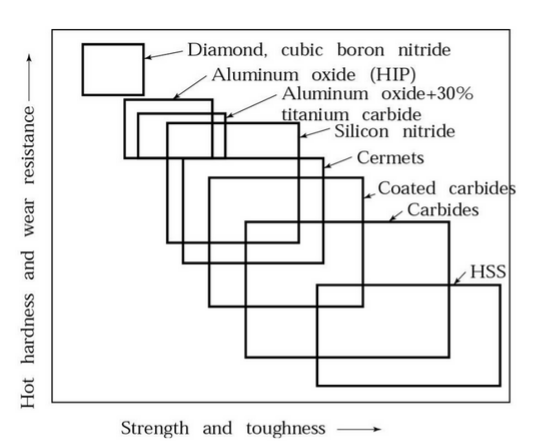
\includegraphics[width = 0.5\textwidth]{MaterialiUtensili}
\caption{Range di caratteristiche dei principali materiali per utensili}
\label{fig:MaterialiUtensili}
\end{figure}

\subsection{Morfologia degli utensili}
Gli acciai rapidi hanno resilienza tale da permettere la realizzazione di utensili monoblocco. Inoltre il costo rimane basso.
Già coi carburi si possono realizzare degli inserti per via del fatto che costano di più e sono più fragili.
Con gli inserti non raffilabili si girano i vertici in modo da consumarli in tutti i senti.
I taglienti con angolo di spoglia grande dovranno essere raccordati per garantire un usura uniforme.
Per gli inserti costosi o molto fragili vengono realizzate delle unghie applicate all'inserto tramite brasatura.

\begin{table}
\centering
\caption{Confronto tra le morfologie degli utensili e i loro costo}
\label{tab:ConfrontoUtensili}
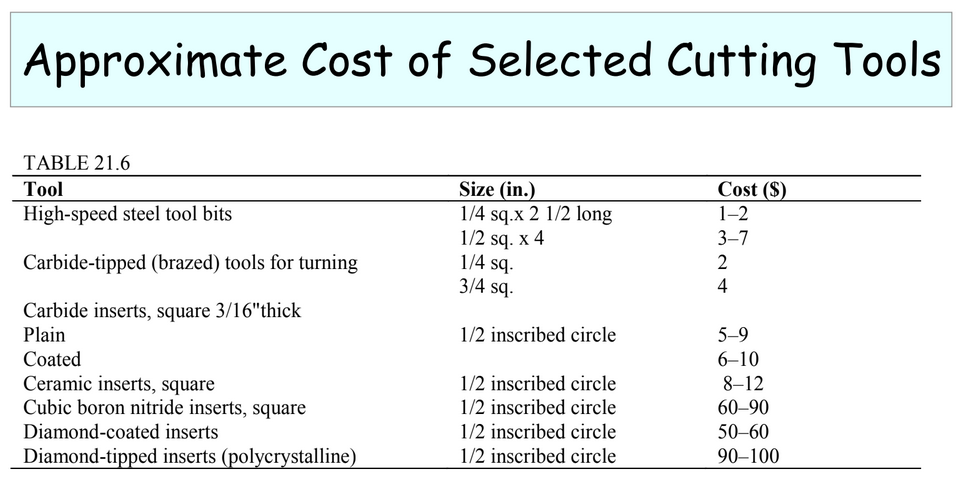
\includegraphics[width = \textwidth]{Utensili}
\end{table}

\subsection{Portautensili e elementi di serraggio}
Il problema di serraggio deve essere fatto in modo che eviti delle vibrazioni che porterebbero a rottura gli utensili.
Ormai grazie alle ai centri \ac{FMS}, che predispongono un proprio magazzino utensili, i portautensili vengono realizzati in modo che siano intercambiabili sul mandrino.
Spesso il cambio utensile viene realizzato tramite un opportuno leveraggio che sposta gli utensili dal magazzino al mandrino.
Alcuni portautensili possono essere predisposti per garantire la fornitura di fluido da taglio in pressione alle cavità dell'utensile.

Forme geometriche snelle sono preferite per limitare le vibrazioni e la facilità d'innesto nella macchina.
In più si evita la flessione di tutto il sistema.

\subsection{Lavorazioni}
Le principali lavorazioni ad asportazione di truciolo sono classificate in base alla quantità di utensili taglienti che contemporaneamente sono immersi nel materiale.
Il grafico \ref{fig:LavAsp} mostra le varie classificazioni.

\begin{figure}
\centering
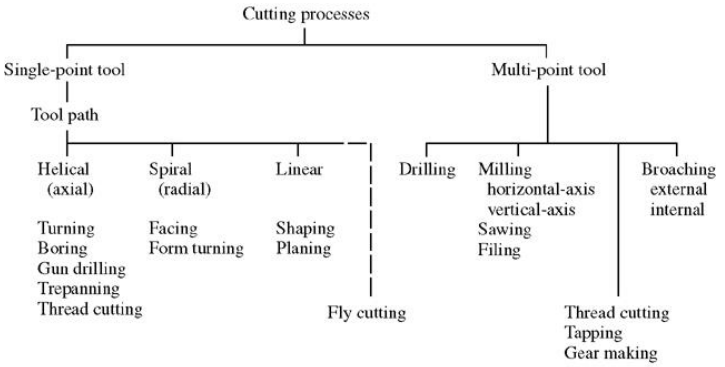
\includegraphics[width = \textwidth]{LavAsp}
\caption{Suddivisione delle principali lavorazioni in asportazione di truciolo}
\label{fig:LavAsp}
\end{figure}

Fanno eccezione le lavorazioni di forma in cui i taglienti sono plurimi ma non rientrano nella classificazione dei taglienti plurimi. Si dicono di forma per l'appunto.
La figura \ref{fig:ShapeTool} riporta degli esempi di utensili di forma.

\begin{figure}
\centering
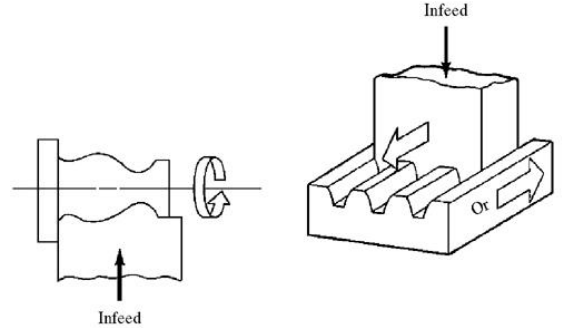
\includegraphics[width = \textwidth]{ShapeTool}
\caption{Alcuni esempi di utensili di forma}
\label{fig:ShapeTool}
\end{figure}

\chapter{Tornitura}
\begin{wrapfloat}{figure}{O}{0pt}
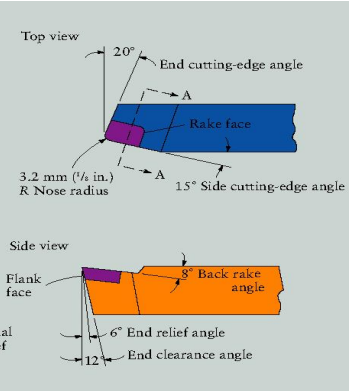
\includegraphics[width = 0.4\textwidth]{ToolAngles}
\caption{Schematizzazione degli angoli per un'utensile da tornitura}
\label{fig:ToolAngles}
\end{wrapfloat}

Si sfrutta un'utensile monotagliente ma la qualità sta nella bravura del operatore.
Di fatto è la prima rappresentazione applicativa di taglio obliquo.
Gli angoli di riferimento sono dipendenti dall'inclinazione del utensile rispetto al pezzo in lavorazione, come si vede dalla figura \ref{fig:ToolAngles}.
Esiste una norma che definisce nel dettaglio gli angoli di riferimento.
Nella rettifica si sfrutta un disco rotante piuttosto che far ruotare il pezzo.
Ciò per dire che il mandrino può mettere in rotazione sia il pezzo che eventuali utensili.

\section{Tornitura cilindrica}
\begin{figure}
\centering
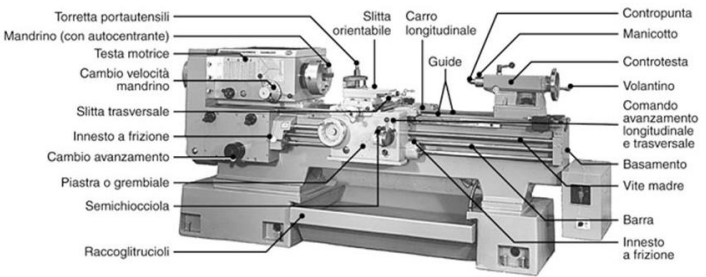
\includegraphics[width = \textwidth]{Turning}
\caption{Specifiche di un tornio classico}
\label{fig:Turning}
\end{figure}
Data la varietà di lavorazioni fattibili con la tornitura, è possibile che i torni presentino ulteriori supporti, dette mezzelune, per impedire la flessione dei lavorati particolarmente lunghi o cedevoli.
In più anche la presenza della contropunta permette di mantenere in asse il pezzo, però resta il limite della flessione imposta dall'utensile stesso.

Di seguito vengono riportate ulteriori lavorazioni possibili al tornio.

\begin{figure}
\centering
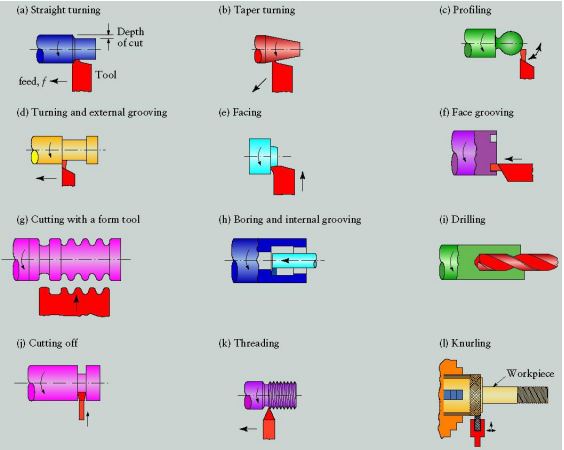
\includegraphics[width = \textwidth]{OtherTurning}
\caption{Ulteriori lavorazioni ottenibili tramite tornitura}
\label{fig:OtherTurning}
\end{figure}

Nello specifico:
\begin{description}
\item[Barenatura] viene usata per allargare dei fori, finire interiormente i fori o se ne modifica la forma.
Il tema è l'utensile: essendo che deve entrare profondamente nel foro questo può essere molto lungo, cioè può essere sottoposto a flessione. Risultando in una finitura peggiore.
\item[Troncatura] Nel caso si voglia separare una parte di materiale in tornitura, l'utensile presenterà più taglienti.
In più si presenta un'ulteriore problema: la velocità angolare di taglio cambia in funzione del raggio a cui si sta lavorando, infatti:
\begin{equation}
v_c = \omega \cdot r \Rightarrow Se r \rightarrow 0 \: v_c \rightarrow 0
\end{equation}
Quando ci si avvicina all'asse di rotazione la qualità superficiale peggiora.
\item[Lavorazioni di forma] Siccome la forza applicata è considerevole si preferisce tenere uno sbalzo limitato.
\item[Limatura e piallatura] Realizzano delle superfici piane, non c'è un moto di rotazione ma di traslazione. In questo caso l'utensile è a sbalzo che può essere problematica.
Cambia solo il moto relativo ma non il risultato.
\end{description}

In generale è da evitare troppi fissaggi per il fatto che possono introdurre distorsioni nel lavorato.

\section{Altre tipologie di torni}
\begin{description}
\item[Torni automatici] È una macchina automatica in grado di eseguire in modo molto rapido la stessa operazione. è sparita perché mancante di versatilità: dunque sostituiti con i centri di lavoro \ac{CNC}.
\item[Torni per viti] Vengono usati per realizzare forme parecchio complicate, anche se ormai la viteria viene realizzata per deformazione plastica a meno di filettature a diverse specifiche.
\item[Torni svizzeri] Hanno deflessioni molto piccole per garantire toleranze molto piccole $\approx 2.5\unit{\um}$. Ciò è possibile grazie a utensili posti su più assi e regolati molto accuratamente.
\end{description}

\chapter{Lavorazioni al trapano}\label{chp:LavTrapano}
È una macchina utensile molto diffusa.
In realtà realizza una sola lavorazione: crea dei fori.
Data la necessità di creare dei fori, se ne capisce la fondamentalità.

\begin{figure}
\centering
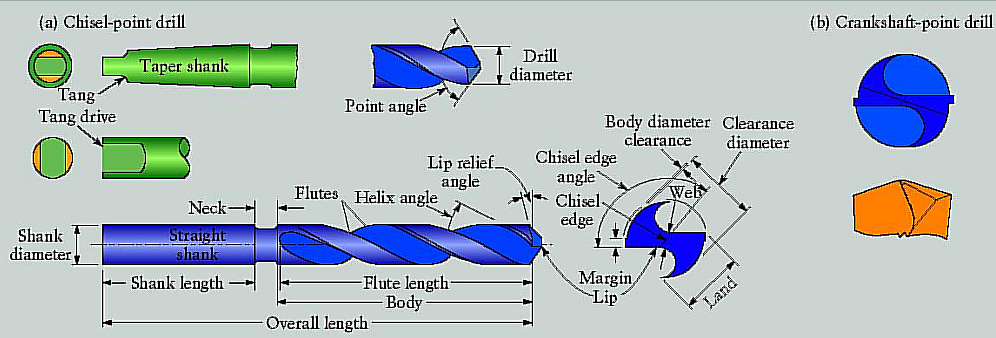
\includegraphics[width = \textwidth]{Trapanatura}
\caption{Alcune punte da trapano per diverse forature}
\label{fig:Tapanatura}
\end{figure}

dalla figura \ref{fig:PunteTrapano} si può vedere che esistono diverse punte da trapano.
Si può già fare un confronto tra le punte da trapano e gli utensili
monotagliente visti per il tornio.
In genere l'utensile monotagliente tende a flettere parecchio, mentre nelle punte da trapano 
le forze sono bilanciate per via della forma del tagliente.
In più le punte presentano delle scanalature elicoidali che dovrebbero assolvere
a due funzioni:
\begin{itemize}
\item rimuovere il truciolo dalla zona di taglio
\item favorire la lubbrificazione del tagliente
\end{itemize}
In realtà non fanno correttamente nessuna delle due operazioni.

\begin{figure}
\centering
\subfloat[][\emph{Principali punte da trapano}
\label{fig:PunteTrapano}]
{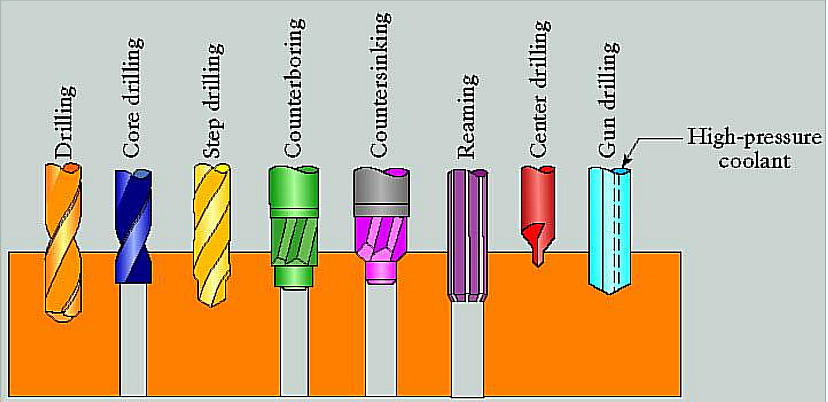
\includegraphics[width = \textwidth]{PunteTrapano}}\\
\subfloat[][\emph{Punte per foratura}\label{fig:PunteForatura}]
{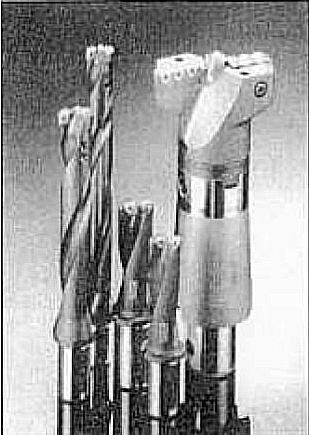
\includegraphics[width = 0.4\textwidth]{PunteForatura}}\quad
\subfloat[][\emph{Esempi di mecchie}\label{fig:UlterioriPunte}]
{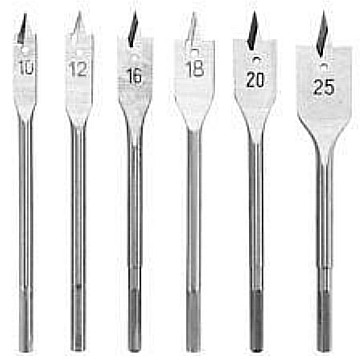
\includegraphics[width = 0.4\textwidth]{UlterioriPunte}}
\caption{Varie tipologie di punte da trapano}
\label{fig:Punte}
\end{figure}

Nella foratura le forze sono bilanciate. Più importante è da considerare:
Man mano che ci si avvicina all'asse della punta i taglienti lavorano ad una velocità di taglio
moinore, per cui la finitura superficiale peggiora.
È per questo motivo che i talgienti delle punte da trapano non arrivano al centro della punta.
Dunque la punta è realizzata con forma conica in modo tale da spostare il materiale in lavorazione 
verso le zone di lavorazione laterali. Insomma funge da scalpello allontanando il materiale
dall'asse di rotazione. Saranno dopo i taglienti ad asportarlo effettivamente. 
Tra l'altro, la forza per spostare il materiale è la maggiore parte di forza utilizzata per tale lavorazione.
Infatti di solito si utilizza prima una foratura più fina per una prima asportazione, poi viene 
eseguita la foratura principale che porta il foro alla dimensione desiderata.

Ovviamente lo scalpello della punta si usura e dunque si dovrà applicare maggiore forza alla punta.
Per cui la forma dello scalpello si è evoluta in modo da rendere minore la forza di spinta da applicare alla 
punta. In più, sulle scanalature elicoidali sono presenti delle scanalature ulteriori che fungono da 
rompitruciolo.

Ulteriore problematica è quella dello spostamento dell'asse della punta. Allora si utilizza una punta
da centri per "indicare" alla punta da trapano la direzione di foratura.

L'angolo dell'elica rappresenta l'angolo di spoglia periferica della punta.
L'angolo di spoglia diminuisce avvicinandosi al centro della punta.
Per favorire lo spostamento del truciolo, spesso si utlizzano delle punte con angolo d'elica particolarmente 
elevato.

Dove c'è dello spazio grigio indica il fatto che si deve eseguire un prima foratura prima di usare 
quell'utensile.

Con riferimento alla figura \ref{fig:PunteTrapano}, rispettivamente sono:
\begin{enumerate}
\item Punta da trapano classica;
\item Va usato dopo l'utensile precedente e semplicemente allarga il foro
\item Realizza un foro a due diametri detta anche \emph{step-drilling}
\item Realizza un gradino su un foro già realizzato, viene detta anche \emph{lamatura}
\item Stesso obbiettivo della precedente \emph{Utensile a lamare}
\item stesso del precedemnte \emph{Utensile a svasare}
\item Utensile di \emph{alesatura} va semplicemente a rifinire il foro fatto in precedenza.
\item Punta da centri, realizza un piccolo for perguidare la punta da trapano.
\item È un utensile utilizzato in particolare per lavorazioni su lamiere.
\end{enumerate}

In genereale le punte da trapano sono degli utensili di materiali monoblocclo. Esistono anche delle punte
da trapano che presentano degli inserti. Certo si hanno dei fori un po' magiori per via delle dimensioni
degli inserti.
Eventualmente si ricorre a dei trattamenti termochimici per aumentare la durata della punta.

Ulteriori utensili sono mostrati in figura \ref{fig:UlterioriPunte}.
Le Mecchie sono utilizzate per realizzare fori di piccola profondità.
Le mecchie di forma conica permettono di realizzare dei fori in base alla profondità a cui si spinge la punta
a diametro variabile. Spesso usate per lavorazioni su lamiere.

\begin{figure}
\centering
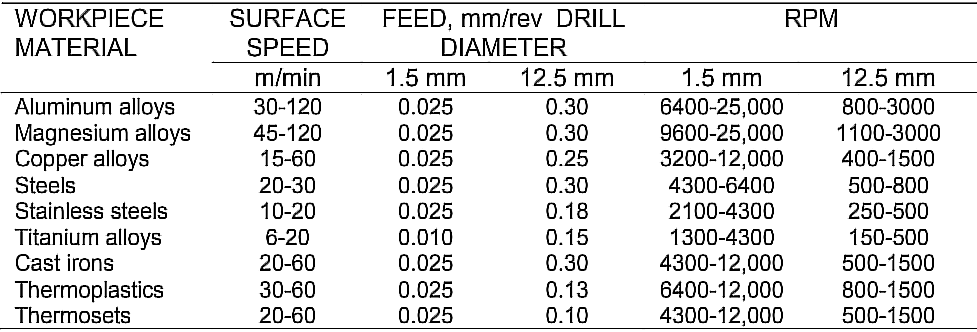
\includegraphics[width = \textwidth]{VelTrapanatura}
\caption{Velocità consigliate di trapanatura}
\label{fig:Veltrapanatura}
\end{figure}

\section{Tipologie di trapani}

\begin{figure}
\centering
\subfloat[][\emph{Esempio di trapano semplice}\label{fig:Trapano}]
{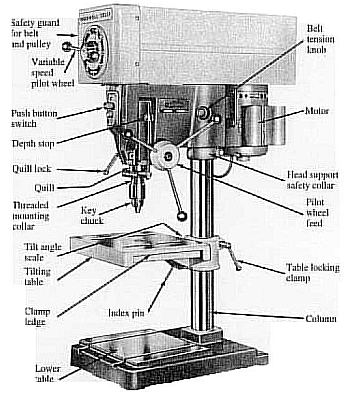
\includegraphics[width = 0.4\textwidth]{Trapano}}\quad
\subfloat[][\emph{Esempio di trapano a controllo numerico}\label{fig:TrapanoCNC}]
{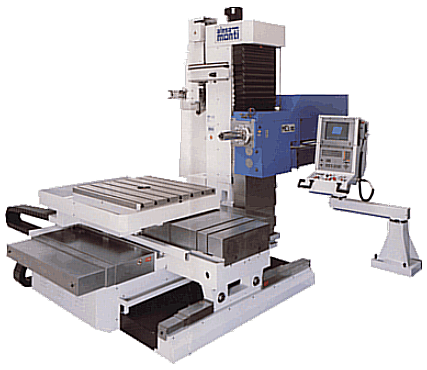
\includegraphics[width = 0.4\textwidth]{TrapanoCNC}}\\
\subfloat[][\emph{Particolare sulle punte alesatrici}\label{fig:PuntaFresatrice}]
{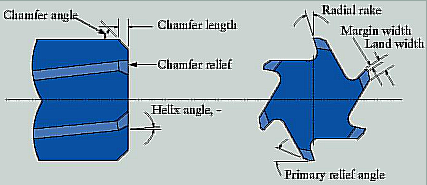
\includegraphics[width = 0.5\textwidth]{PuntaFresatrice}}
\caption{Alcuni esempi di trapani e dettaglio punta alesatrice}
\label{fig:Trapani}
\end{figure}
Alcuni esempi di trapanio sono riportati alle figure \ref{fig:Trapani}. Risulta molto riduttivo parlare di macchine che eseguono solo trapanature (nonostante esistano e vengano tutt'oggi prodotte) perché ormai soppiantate dai centri di lavoro \ac{FMS}.
Di fatto l'evoluzione dei centri \ac{FMS} ha ormai inglobato quasi tutte le possibili lavorazioni per asportazioni di truciolo in un'unica macchina.
Di questo se ne parlerà nel capitolo \ref{chp:MacchineUtensili} a pagina \pageref{chp:MacchineUtensili}.

Piccolo approfondimento per le punte da alesaggio.\\
Le punte da alesaggio \ref{fig:PuntaFresatrice} hanno scanalature piccole, questo perché si ha meno materiale da rimuovere, in più si ha una maggiore rigidezza dell'utensile per via del maggiore spessore del centro.
In generale gli utensili alesatori hanno angoli di elica sono molto molto piccole o addirittura cilindriche.

\chapter{Fresatura}\label{chp:Fresatura}
È la lavorazione più versatile che si può trovare in officina, permette di realizzare la più grande varietà di forme.
Un esempio è quello della fresatrice orizzontale: \ref{fig:FresaOrizzontale} determinato dall'asse di rotazione dell'utensile.
\begin{wrapfloat}{figure}{O}{0pt}
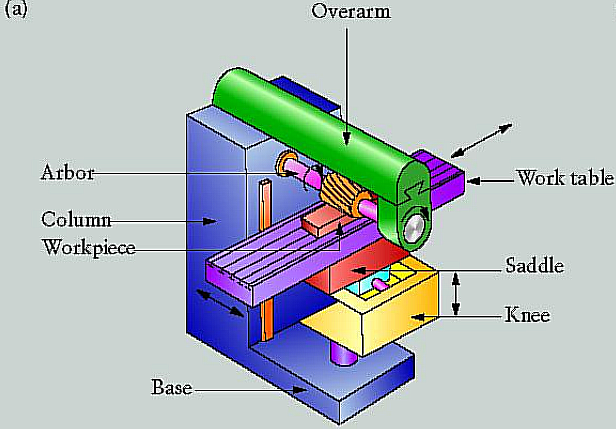
\includegraphics[width = 0.4\textwidth]{FresaOrizzontale}
\caption{Esempio di fresatrice orizzontale}
\label{fig:FresaOrizzontale}
\end{wrapfloat}
L'utensile può presentare taglienti elicoidali sia cilindrici.

Siccome la varietà di lavorazioni è alta, anche la gamma di utensili è piuttosto ampia.

L'evoluzione della lavorazione ha portato al fatto che gli utensili non sono sostenuti da due "cerniere".
Piuttosto si utilizzano utensili fissati a singolo punto.
Il tipo ideale di fresatura si chiama \emph{fresatura periferica}.

\section{Fresatura periferica}
Come anticipato, l'utensile può essere ad elica o a scanalature cilindriche. In genere si preferisce il tagliente ad elica perché subisce meno urti e si possono avere più taglienti immersi sul materiale contemporaneamente.
 
Le eliche possono essere in concordanza \ref{fig:FresaConc} o opposizione \ref{fig:FresaOpp}.
La differenza, oltre che alle direzioni di lavorazione e alimentazione sta anche nel metodo di asportazione. 
Infatti nella lavorazione in concordanza il tagliente, in figura \ref{fig:TaglConc}, incontra immediatamente la superficie del lavorato. Ciò provoca urti più alti al tagliente e in potrebbe incontrare pure degli ossidi che rendono il materiale più duro.

Mentre la lavorazione in opposizione, figura \ref{fig:TaglOpp}, presenta un problema di deformazione elastica: siccome lo spessore indeformato è nullo, il tagliente andrà a schiacciare il materiale andandolo a subire il successivo comportamento elastico.

\begin{figure}
\centering
\subfloat[][\emph{Fresatura in opposizione}\label{fig:FresaOpp}]
{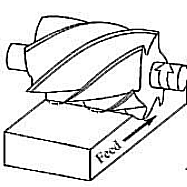
\includegraphics[width =0.4\textwidth]{FresaOpp}}\quad
\subfloat[][\emph{Fresatura in concordanza}\label{fig:FresaConc}]
{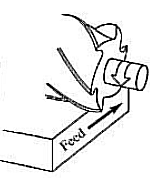
\includegraphics[width = 0.4\textwidth]{FresaConc}}\\
\subfloat[][\emph{Dettaglio del tagliente in opposizione}\label{fig:TaglOpp}]
{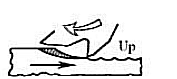
\includegraphics[width = 0.4\textwidth]{TaglOpp}}\quad
\subfloat[][\emph{Dettaglio del tagliente concorde}\label{fig:TaglConc}]
{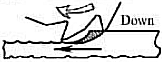
\includegraphics[width = 0.4\textwidth]{TaglConc}}
\caption{Fresatura in opposizione e concordanza}\label{fig:DirFresa}
\end{figure}

In generale si sfrutta la fresatura in concordanza nel caso in cui si predilige una migliore finitura superficiale e il materiale non è stato trattato a caldo: per cui non presenta ossidi superficiali che potrebbero consumare molto rapidamente i taglienti.
Altrimenti si sfrutta la fresatura in opposizione al netto delle peggiori tolleranze dimensionali ottenibili per via del ritorno elastico e la maggiore rigidezza della macchina necessaria per via dello scambio di forze che si va a verificare durante la lavorazione.

La lavorazione in definitiva viene detta anche \emph{spianatura}. 
A differenza di quanti visto per la piallatrice o levigatrice, la lavorazione risulta più veloce in quanto non è necessaria la corsa di ritorno e l'utensile può essere parecchio largo.

La spianatura può essere realizzata anche tramite utensile a sbalzo monotagliente.

\section{Fresatura verticale}
In questo caso si ha l'asse dell'utensile in verticale rispetto al lavorato. 
Attenzione che l'utensile è a sbalzo e non più fissato a due punti, quindi generalmente più rigido.
Può essere che queste macchine sfruttino una tecnologia ibrida per cui possono realizzare sia lavorazioni
in verticale che in orizzontale.
\begin{wrapfloat}{figure}{I}{0pt}
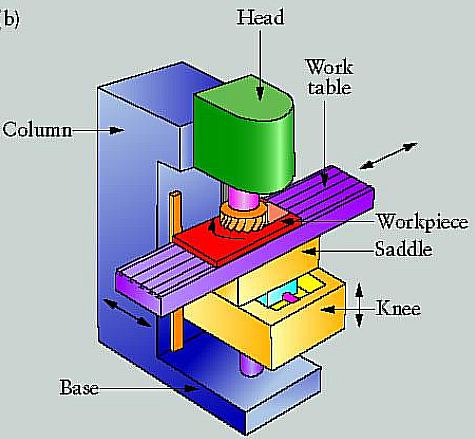
\includegraphics[width = 0.4\textwidth]{FresaVert}
\caption{Esempio di fresa verticale}
\label{fig:FresaVert}
\end{wrapfloat}

\begin{quote}
\emph{Come mai si preferisce un'utensile a sbalzo rispetto ad uno più rigido magari fissato in due punti?}
\end{quote}

È più facile cambiare utensile e può essere fatto automaticamente. Anche l'accessibilità alla zona di lavoro
non è da sottovalutare.
L'affermazione di tali macchinari è, dunque, puramente pratico.
Per cui si preferisce che l'utensile sia a sbalzo.

\subsection{Fresa a codolo}
La fresa a codolo, in figura \ref{fig:FresaCodolo}, è molto simile ad un trapano, ma la punta non presenta lo scalpello in virtù del fatto che l'elica non ha lo scopo di effettuare una foratura. Bensì l'elica ha lo scopo di evitare degli urti del tagliente che teoricamente potrebbe essere perfettamente cilindrico.
La tipica lavorazione di questa macchina è l'ottenimento di oggetti a piani paralleli.
Si ottengono dei gradini per via della lavorazione a piani paralleli, quindi sarà necessaria una successiva passata di finitura per ottenere una forma continua.
Tra l'altro, i piani non per forza devono essere orizzontali, possono essere anche verticali o a diversa inclinazione.
Indubbiamente l'automazione di queste macchine è fondamentale. Le quali possono realizzare delle forme che non sarebbero ottenibili con altre macchina.
In generale macchine ad alta automazione vengono anche chiamate \emph{centro di lavoro}.
Sono delle macchine ad alta automazione che uniscono i vantaggi delle principali lavorazioni per asportazione di truciolo.
Realizzano lavorazioni su tutte e 5 le facce del pezzo (La faccia di riferimento è quella appoggiata al porta-pezzo). In inglese \ac{FMS}.

Una prodotto tipico di queste lavorazioni sono gli stampi.

\begin{wrapfloat}{figure}{O}{0pt}
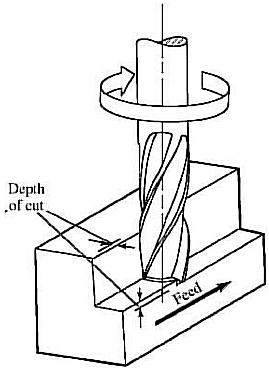
\includegraphics[width = 0.3\textwidth]{FresaCodolo}
\caption{Schematizzazione della fresatura a codolo}
\label{fig:FresaCodolo}
\end{wrapfloat}

Per ridurre tale condizione, evitando di fare più passate successive, si possono usare delle frese a codolo a testa sferica, \ref{fig:FresaSferica}, che evitano il problema della velocità radiale nulla al centro della punta. Vanno usate ad un'inclinazione di circa $15\unit{\degree} \div 30\unit{\degree}$ per mantenere una buona velocità radiale in qualsiasi punto dei taglienti. 

\begin{figure}
\centering
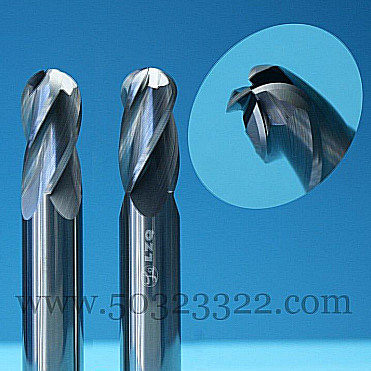
\includegraphics[width = 0.4\textwidth]{FresaSferica}
\caption{Esempio di frese a testa sferica}
\label{fig:FresaSferica}
\end{figure}

\section*{Il controllo numerico}
\begin{description}
\item[Asse controllato] quando di quell'asse se ne può controllare posizione e velocità
\end{description}

\begin{quote}
Quanti assi controllati per ogni tipo di lavorazione?
\end{quote}

Per il trapano ad esempio è sufficiente un solo asse, l'avanzamento della punta.
Per il tornio ne bastano due: uno in direzione ortogonale all'asse di rotazione del pezzo e uno in direzione 
parallela.
Per la fresatrice invece sono 3.

Negli assi mandrino, si controllano solamente la velocità quindi non viene considerato come asse controllato.

Quando si parla di macchine a più assi (4,5) si possono avere delle rotazioni dell'utensile.
Eventualmente Si possono sfruttare degli utensili a testa sferica (opportunamente inclinati per non avere 
velocità nulle sull'asse di rotazione).

\chapter{Altre Lavorazioni}\label{chp:AltreLav}
\section{Taglio con sega}
Risulta una forma di fresatura, con dei taglienti molto fini.
In genere si sfrutta un'utensile cilindrico molto fino al quale vengono
attaccati i taglienti che possono essere di materiale diverso da quello 
dell'utensile stesso.
Viene spesso utilizzata per separare due parti di materiale.
In figura \ref{fig:Seghe} ne sono presentate alcune.

\begin{figure}
\centering
\subfloat[][\emph{Tipologie principali di seghe utilizzate in industria}
\label{fig:Seghe}]
{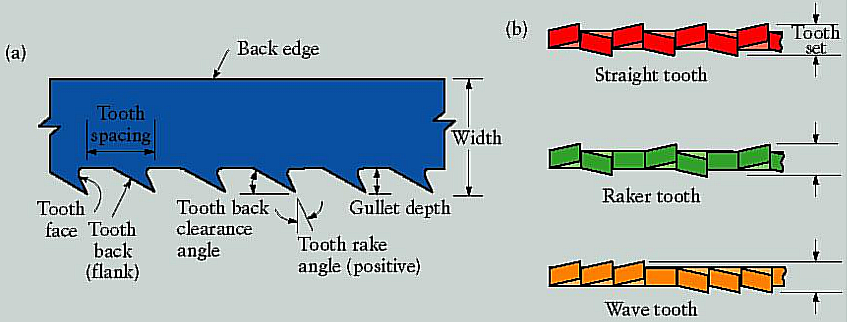
\includegraphics[width = \textwidth]{Seghe}}\\
\subfloat[][\emph{Esempio di inserto per sega}\label{fig:SegheInserti}]
{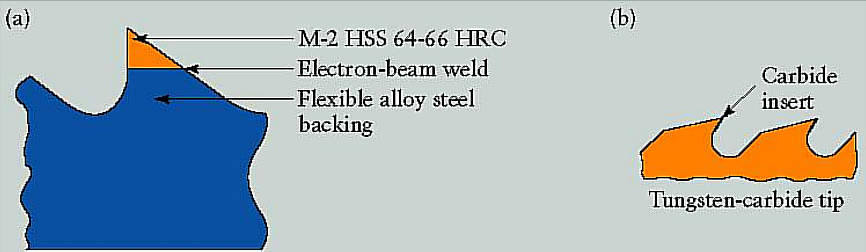
\includegraphics[width = \textwidth]{SegheInserti}}
\caption{Breve descrizione delle seghe industriali}
\label{fig:SegheInd}
\end{figure}

\section{Brocciatura e taglio di filetti}
\subsection{La brocciatura}
si ha sempre un'utensile di forma, di cui se ne controlla solo il moto primario. Ciò è possibile perché l'avanzamento viene realizzato per cui
sarà il tagliente ad avanzare autonomamente.
La maggior parte del materiale verrà asportata di taglienti detti di sgrossatura per poi essere finiti dai taglienti di finitura.
Ad ogni componente da realizzare il suo utensile.

Solitamente si eseguono dei fori non circolari. Si effettua da prima 
un foro circolare per poi passare con la \textit{broccia}, in figura \ref{fig:Broccia}, che realizza forme particolare come richiesto.

\begin{figure}
\centering
\subfloat[][\emph{Esempio e parametrizzazione di una broccia}\label{fig:Broccia}]
{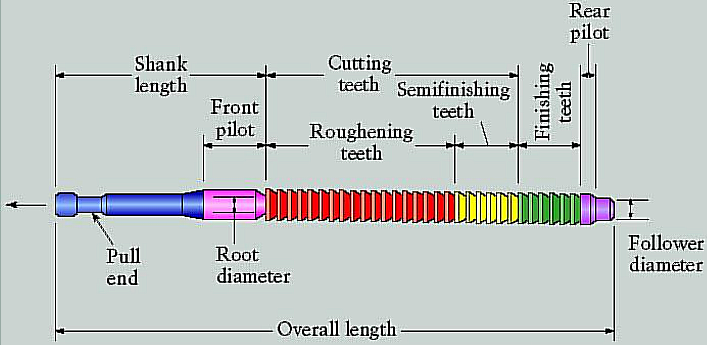
\includegraphics[width = \textwidth]{Broccia}}\\
\subfloat[][\emph{Dettaglio della lavorazione tramite broccia}
\label{fig:DettaglioBroccia}]
{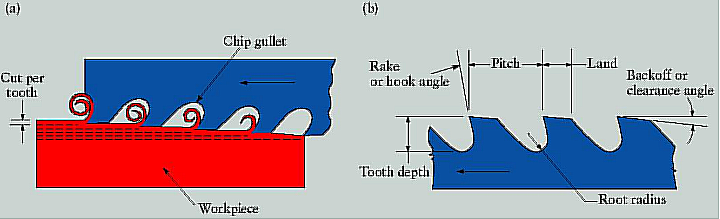
\includegraphics[width = \textwidth]{DettaglioBroccia}}
\caption{Brocciatura}
\label{fig:Brocciatura}
\end{figure}

Si tratta di un utensile parecchio costoso per via del fatto che è un'utensile massiccio. Viene utilizzato solitamente per la produzione in grande serie, per ammortizzare meglio il costo.
I taglienti asportano il materiale in maniera progressiva, in figura \ref{fig:DettaglioBroccia}, a differenza di quanto visto per altri utensili precedenti.
Da considerare l'eventuale deflessione dell'utensile posta dalla resistenza
meccanica del materiale lavorato, soprattutto per brocciature esterne.
Per quelle interne non sussiste il problema.
La boccia può essere spinta nel materiale oppure tirato.
Se spinto si sfruttano delle brocce piuttosto corte per via dell'ampia
deflessione che si va a generare.
Discorso diverso nel caso in cui l'utensile viene tirato, per cui si possono avere brocce fino a $2\unit{\m}$.

\subsection{Filettature}
L'operazione non è molto diversa da quella precedente: cambia il tipo di moto applicato all'utensile: nella filettatura si ha un moto di rotazione
elicoidale per cui l'utensile avanza radialmente e longitudinalmente.

\begin{figure}
\centering
\subfloat[][\emph{Utensile per filettatura interna}\label{fig:FilettaturaEsterna}]
{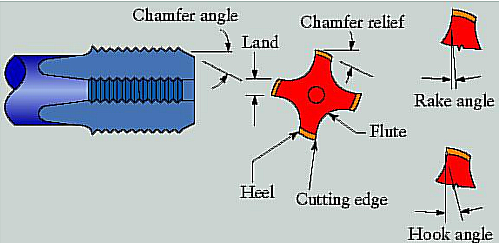
\includegraphics[width = 0.4\textwidth]{FilettaturaInterna}}\quad
\subfloat[][\emph{Utensile per filettatura esterna}]
{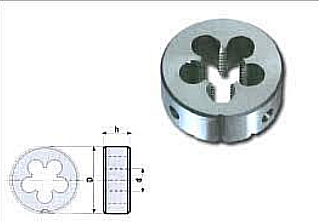
\includegraphics[width = 0.4\textwidth]{FilettaturaEsterna}}
\caption{Utensili per filettature}
\label{fig:Filettature}
\end{figure}

Normalmente la filettatura viene realizzata tramite deformazione plastica,
si ha incrudimento per lavorazione a freddo, non si asporta materiale e dunque le fibre del materiale non vengono tagliate orientandole in senso
assiale rispetto alla filettatura dando ulteriore resistenza meccanica.

\section{Aspetti conclusivi}
Alla figura \ref{fig:TolleranzeFiletti}, vengono riportate quali sono le principali lavorazioni ottenibili per asportazione di truciolo. Vengono anche specificate le tolleranze minime ottenibili.
Mentre alla figura \ref{fig:ProductionRates}, sono indicati quali siano le produttività.
\begin{figure}
\centering
\includegraphics[width = \textwidth]{TolleranzeFiletti}
\caption{Riepilogo lavorazioni per asportazione di truciolo}
\label{fig:TolleranzeFiletti}
\end{figure}
\begin{figure}
\centering
\includegraphics[width = \textwidth]{ProductionRates}
\caption{Indicazioni sulla produttività delle specifiche lavorazioni per asportazione di truciolo}
\label{fig:ProductionRates}
\end{figure}

\section{Produzione di ingranaggi}\label{sc:Ingranaggi}
Per la produzione di ingranaggi si sfruttano quasi tutte le lavorazioni che si sono viste in precedenza come evidenziato dalla figura \ref{fig:Ingranaggi}.
In particolare, gli ingranaggi per applicazioni critiche, sono ancora realizzati tramite lavorazioni per asportazione di truciolo. Ciò garantisce un'ottima finitura di forma, arrivando a tolleranze molto restrittive.
Spesso sono lavorazioni di forma, con moto alternativo (caso della lamatura), oppure rotativo (caso della fresatura).

\begin{figure}
\centering
\includegraphics[width = \textwidth]{Ingranaggi}
\caption{Alcuni utensili per la produzione di ingranaggi}
\label{fig:Ingranaggi}
\end{figure}

Più complicata è la realizzazione di ingranaggi conici.
Si devono utilizzare degli utensili di forma, su macchine più adatte per 
tale scopo.